\chapter{Introdu\c{c}\~{a}o}

A indústria de jogos digitais é um dos segmentos de entretenimento mais rentáveis do mundo atualmente, superando, por exemplo, a indústria do cinema e da música \cite{newzoo1} \cite{ifpi1} \cite{mpaa1}. Conforme \cite{newzoo1}, o mercado de jogos digitais alcançou mais de 99,5 bilhões de dólares em 2016. Um fator importante para esse sucesso é a possibilidade de jogar \textit{online} e construir equipes com jogadores de todo o mundo.

Um segmento de jogo muito popular atualmente é o esporte eletrônico, mais conhecido como \textit{eSport} \cite{forbes1}. Conforme \cite{newzoo2}, o mercado de \textit{eSport} alcançou 493 milhões de dólares e uma audiência global de 191 milhões de entusiastas em 2016. O \textit{eSport} mais popular e mais rentável do mundo hoje é o League of Legends (LoL)  \cite{superdata1}, desenvolvido pela Riot Games, com cerca de 67 milhões de jogadores ativos e um pico diário de mais de 7,5 milhões de jogadores \textit{online} simultâneos \cite{riot1}.

LoL é um jogo de arena de batalha \textit{online} para vários jogadores (\textit{Multiplayer Online Battle Arena} - MOBA), um subgênero de jogos digitais de estratégia em tempo real (\textit{Real-time Strategy} - RTS). Uma partida em um MOBA consiste em um cenário (mapa) em que duas equipes lutam entre si, a fim de destruir a base do oponente como o principal objetivo, sem limite de tempo. Um mapa simples contém três estradas principais (rotas) que conectam a base de cada equipe. Em geral, uma equipe tem cinco jogadores e cada um seleciona e controla um personagem, conhecidos como campeões ou heróis, com atributos e habilidades distintas. Além disso, as equipes também contam com a assistência de estruturas de defesa e unidades controladas por Inteligência Artificial (IA), conhecidos como \textit{minions} ou \textit{creeps}, para vencer a partida. Ao longo de uma partida, os personagens ganham ouro - que é usado para comprar itens que melhoraram seus atributos e habilidades - e pontos de experiência de várias maneiras, como matar unidades ou personagens e destruir estruturas da equipe inimiga \cite{league1}.

A grande diversidade e dinamicidade das ações dos personagens nas partidas \cite{drachen2014skill}, bem como seus desempenhos individuais (ou seja, ouro ganho, campeões abatidos ou derrotados, dano causado, cura recebida, etc.), tornam os MOBAs jogos muito competitivos. Em LoL, esta competitividade é ampliada devido à sua popularidade e torneios que fazem com que muitos jogadores se comportem como desportistas profissionais \cite{rioult2014mining}.

Dominar LoL é muito desafiador e requer um investimento substancial de tempo \cite{drachen2014skill}, principalmente para equipes inexperientes que não sabem inicialmente como elaborar ou melhorar sua estratégia. Nesse sentido, uma alternativa que poderia ajudar essas equipes é fornecer informações que levem a melhores decisões estratégicas no jogo. Um exemplo dessas informações poderia ser métricas de desempenho baseadas no comportamento de equipes bem-sucedidas. Com isso, as equipes poderiam monitorar seus desempenhos ao longo das partidas e verificar se estão no caminho correto ou não. Uma das abordagens para o criação de métricas de desempenho é o uso da mineração de dados \cite{el2016game}, que permite o estudo da coleta, preparação, processamento, análise e obtenção de informações úteis a partir de dados para apoiar a tomada de decisões \cite{aggarwal2015data}.

Uma das abordagens para a aplicação da mineração de dados é a utilização do aprendizado de máquina \cite{aggarwal2015data}, uma subárea da IA que explora o estudo e construção de algoritmos que permitem ao computador aprender utilizando dados. Os algoritmos de aprendizado de máquina fazem uso do princípio de inferência chamado indução, com o qual é possível obter conclusões genéricas a partir de um conjunto de dados fornecido \cite{lorena2007introduccao}. Esse aprendizado indutivo pode ser dividido em dois tipos principais: supervisionado e não supervisionado. No aprendizado supervisionado uma máquina é treinada com base em um conjunto de dados onde os rótulos das observações são previamente conhecidos para realizar tarefas de previsão, classificação e regressão, já no aprendizado não supervisionado não existem observações rotuladas para que a máquina possa aprender sobre o domínio do problema, e seu objetivo é descobrir padrões ou características nos dados \cite{sathya2013comparison} por meio de métodos de agrupamento, associação, estimação de densidade, dentre outros.

No contexto de análise de comportamento de jogadores, onde tipicamente não se tem certeza de como o comportamento pode variar, os algoritmos de aprendizado de máquina fornecem meios para descobrir as principais características nos dados e padrões relacionados ao comportamento em função dessas características \cite{el2016game}. Esses padrões podem ser utilizados para caracterizar os perfis das equipes, ou seja, equipes que possuem comportamento similar, bem como classificar o perfil de uma equipe.

\section{Objetivos}
Esta dissertação tem como objetivo apresentar e discutir os resultados de um processo de mineração de dados para identificar e caracterizar perfis de comportamento de equipes bem-sucedidas e malsucedidas no contexto do jogo League of Legends, baseando-se em métricas sumarizadas de desempenho dos jogadores nas partidas. Para atingir o objetivo, primeiro, coletamos partidas do \textit{site} oficial de histórico de partidas de LoL. Em seguida, modelamos um conjunto de dados de desempenho de equipes extraindo características a partir de estatísticas básicas de desempenho individual dos jogadores nas partidas, como quantidade de ouro ganho, quantidade de monstros abatidos, dano físico total recebido, dentre outros. Depois, para transformar os dados em métricas úteis de desempenho, realizamos outras tarefas relacionadas a preparação de dados, tais como limpeza de dados, remoção de características com baixa variância, detecção de \textit{outliers}, transformação de dados, normalização de dados e análise de redundância de características. Para descobrir padrões de comportamento, aplicamos uma análise de agrupamento (\textit{K-means clustering}) nos dados desempenho de equipes para descobrir um número ótimo de grupos e, assim, agrupar equipes similares. Finalmente, caracterizamos cada grupo por meio de uma análise exploratória dos dados. Os resultados implicam que alguns grupos de equipes são mais propensos a terem equipes vencedoras do que outros e a influência das características é distinta para cada um, o que nos permitiu definir perfis de equipes bem-sucedidas e malsucedidas baseando-se nas métricas de desempenho das equipes.

\subsection{Questões de Pesquisa}

\begin{enumerate}[label=(\roman*)]
  \item É possível computar métricas de desempenho de equipes?
  \item É possível encontrar padrões úteis no comportamento das equipes com base nessas métricas?
  \item É possível caracterizar perfis de comportamento de equipes bem-sucedidas e malsucedidas usando esses padrões?
\end{enumerate}

\section{Contribuições}
Acreditamos que este trabalho resultou em uma importante contribuição ao unir o tema comportamento de usuários aos jogos MOBA. Esses jogos possuem uma crescente popularidade e uma série de aspectos a serem estudados. Até onde sabemos, ainda existe uma escassez de trabalhos acadêmicos que os exploram \cite{drachen2014skill} \cite{ong2015player}, especialmente em relação ao comportamento de jogadores e equipes em LoL.

Podemos identificar ao menos três classes principais de \textit{stackholders} para as quais os resultados desta pesquisa são relevantes. Primeiro, a comunidade de mineração de dados, pois este trabalho representa um domínio novo e ainda pouco explorado. Em segundo lugar, a indústria de jogos digitais que pode se beneficiar dos modelos descritivos e preditivos desenvolvidos para compreender melhor os jogadores e as equipes e, assim, fornecer ferramentas automáticas para melhorar a experiência de jogo. Finalmente, jogadores e equipes inexperientes que podem se beneficiar das informações obtidas a partir dos perfis de equipes bem-sucessidadas e malsucedidas para apoiar suas decisões e, assim, melhorar suas habilidades, tornando o jogo ainda mais divertido.

Por fim, este trabalho também resultou na aceitação do artigo científico "\textit{Profiling Successful Team Behaviors in League of Legends}" no XXIII Simpósio Brasileiro de Sistemas Multimídia e Web (WebMedia 2017). Nesse artigo, foram abordados os temas e experimentos aqui tratados, sendo este trabalho uma extensão mais aprofundada do artigo.

\section{Estrutura da Dissertação}
Esta dissertação encontra-se dividida em 7 capítulos. O Capítulo 2 apresenta uma introdução sobre o histórico dos MOBAs e uma fundamentação teórica sobre mineração de dados. O Capítulo 3 apresenta os trabalhos relacionados, abordando os temas necessários ao desenvolvimento deste trabalho sobre MOBAs e aprendizado de máquina de uma maneira geral. O Capítulo 4 apresenta os resultados da metodologia adotada para preparar os dados de desempenho das equipes que foram usados nas análises. O Capítulo 5 apresenta os resultados da análise de agrupamento que foi usado para encontrar padrões ou grupos nos dados. O Capítulo 6 apresenta a caracterização de perfis conforme os grupos ou padrões encontrados. O Capítulo 7 finaliza este trabalho com as conclusões e trabalhos futuros.

\chapter{Fundamentação Teórica}

Este capítulo aborda o histórico dos MOBAs e os principais conceitos relacionados a mineração de dados no contexto de jogos digitais.

\section{MOBA}
Os jogos MOBA tem suas origens nos jogos do gênero RTS, muito populares em meados dos anos 90 e início dos anos 2000. Suas características herdam traços que estão presentes em ambos os gêneros, sendo que os primeiros MOBAs foram criados utilizando as próprias ferramentas de criação de mapas personalizados RTS disponibilizados pelas desenvolvedoras. Para que se possa entender melhor as origens e características dos jogos MOBA, apresenta-se nesta seção um breve histórico de evolução do gênero.

Assim, com a popularidade dos jogos de estratégia, houve grande interesse por parte dos jogadores em criar modos de jogo e mapas personalizados para estes, denominados de \textit{mods}. Esses jogadores se tornaram, portanto, modificadores do conteúdo dos jogos ou \textit{modders}. Os \textit{modders} eram responsáveis pelo desenvolvimento de mapas alternativos, e muitos destes tendiam para o estilo de jogo de um MOBA. Desde o início do desenvolvimento do gênero, a jogabilidade consistia em controlar um personagem denominado "herói" ou "campeão", escolher entre três rotas para avançar suas tropas e conquistar a estrutura principal inimiga.

\subsection{Aeon of Strife}
Um dos primeiros MOBAs de sucesso teve origem no jogo RTS da Blizzard, Starcraft. Em 1998, um \textit{modder} conhecido como Aeon64 criou o Aeon of Strife, um mapa alternativo para o Starcraft. Nele, os jogadores controlavam um único herói cada e lutavam em uma equipe contra outra controlada por IA em três rotas do mapa. Essas rotas conectavam as bases das duas equipes. O objetivo era destruir a base da outra equipe.

Embora \textit{Aeon of Strife} tenha estabelecido os fundamentos para o gênero MOBA, existiam algumas diferenças notáveis do que se espera de um MOBA atualmente. As equipes tinham quatro jogadores cada, em vez de cinco. Além disso, Aeon of Strife não era um jogo competitivo. Em vez disso, uma equipe de personagens controlados por jogadores combatiam contra uma equipe de personagens controladas por IA. Os personagens também não subiam de nível enquanto o jogo progredia, e não existia também uma selva no mapa com monstros e trilhas extras entre as três rotas.

\subsection{Defense of the Ancients}
Após o sucesso de AeoN of Strife, houve outro jogo que chamou a atenção da comunidade \textit{modder}: o também RTS da Blizzard, Warcraft III. Este jogo era essencialmente parecido com Starcraft, porém tinha raças diferentes, gráficos tridimensionais melhores, uma série de cenários novos e ambiente de personalização mais poderoso com suporte a uma linguagem de programação.

Em 2002, a Blizzard lançou seu próximo jogo RTS, o Warcraft III. Este jogo era essencialmente parecido com Starcraft, porém tinha raças diferentes de personagens e monstros, gráficos tridimensionais melhores, uma gama de cenários novos e ambiente de personalização mais poderoso, atrelado inclusive a uma linguagem de programação. Em 2003, um \textit{modder} conhecido como Eul criou um \textit{mod} inspirado no Aeon of Strife chamado Defense of the Ancients. Em breve, outros jogadores criaram sua própria versão de Defense of the Ancients, frequentemente chamado de Dota, cada um adicionando seus próprios heróis, itens e outras diferenças.

Assim como Aeon of Strife, Dota permitiu que os jogadores controlassem uma poderosa unidade de heróis e combatessem uma equipe inimiga em três rotas que ligavam a base de cada equipe. No entanto, Dota fez com que duas equipes de personagens controlados por jogadores competissem uns contra os outros, cada equipe tinha cinco jogadores, os heróis subiam de nível à medida que ganhavam experiência e existia uma selva no mapa cheia de monstros entre as trilhas das rotas. Na prática, é exatamente o que se espera de um MOBA hoje.

Em 2004, um modder conhecido como Guinsoo criou o \textit{mod} Dota Allstars (DotA). Esta versão combinou elementos de múltiplas variações do Dota, e rapidamente se tornou a versão mais popular do mapa. Em 2005, Guinsoo anunciou sua saída do desenvolvimento do \textit{mod}, deixando o desenvolvimento nas mãos de outro \textit{modder} conhecido como IceFrog.

Sob a direção de IceFrog, DotA continuou a crescer em popularidade, pois tornou as partidas do \textit{mod} mais equilibradas. As produtoras inclusive passaram a investir em campeonatos e competições específicas para o DotA. O sucesso foi tamanho que houve a criação de plataformas competitivas, como a Garena, que passaram a dar suporte específico para partidas de DotA.

\subsection{League of Legends}
Dota Allstars ainda era um \textit{mod} para o Warcraft III. Isso significa que ele dependia de todos os recursos desse jogo, de modo que nunca poderia apresentar um personagem que usasse um modelo completamente novo, nem poderia dar a nenhum dos criadores que trabalhavam nisso um lucro monetário.

Devido ao sucesso de DotA, algumas desenvolvedoras resolveram apostar no estilo de jogo. Em 2009, a desenvolvedora Riot Games lançou o League of Legends. LoL é semelhante ao mapa de Warcraft III em estilo e \textit{design}, mas sua estética é um pouco mais cartunesca e a mecânica um pouco mais fácil de entender. Este é o jogo mais jogado do mundo até os dias atuais, tendo superado o jogo World of Warcraft em meados de 2012. Até então o termo MOBA era inexistente e os jogos eram simplesmente denominados \textit{Aeon like}, \textit{DotA like} e \textit{Action Real-Time Strategy}. A Riot Games foi considerada a responsável por cunhar o termo MOBA.

Um ponto importante a notar no LoL é a estrutura de preços. LoL é livre para jogar, o que significa que qualquer um pode fazer o \textit{download} e experimentar o jogo imediatamente, usando uma seleção rotativa de personagens grátis semanal para jogar uma partida. No entanto, se algum jogador quiser um personagem específico para controlar a qualquer momento em um partida, ele tem que comprar. Esse modelo de negócios foi um enorme sucesso quando o jogo foi lançado. As pessoas que nunca fariam o \textit{download} de um \textit{mod} para um antigo jogo de PC como Warcraft III estavam experimentando curiosamente o novo MOBA.

\subsection{Outros}
Além da Riot Games, a Valve resolveu apostar no mercado MOBA, lançando em 2013 uma nova versão do jogo Dota, o Dota2. Neste, os mesmos personagens e jogabilidades de DotA foram mantidos, porém recriados em uma plataforma dedicada e com gráficos melhorados. Outros jogos originados de DotA também ganharam forma, como o Heroes of Newerth (2010), da S2 Games, onde a jogabilidade de DotA foi reproduzida com personagens diferentes. Outros jogos de destaque na atualidade do gênero MOBA são: Smite (2014), da Hi-Rez Studios; Strife (2015), da S2 Games; e Heroes of the Storm (2015), da Blizzard.

\section{Mineração de Dados}
A mineração de dados é o estudo da coleta, preparação, processamento, análise e obtenção de informações úteis a partir de dados. Existe uma grande variação em relação ao domínio de problemas, aplicações, formulações e representações de dados. Portanto, mineração de dados é um termo abrangente que é usado para descrever diferentes aspectos do processamento de dados \cite{aggarwal2015data}.

Atualmente, devido aos avanços tecnológicos e da informatização de todos os aspectos da vida moderna, praticamente todos os sistemas automatizados geram ou armazenam alguma forma de dados. Isso resultou em um crescimento excessivamente rápido do volume de dados, atingindo a ordem de petabytes ou exabytes \cite{aggarwal2015data}.

Esse crescimento excessivo do volume de dados vem emergindo em diversas áreas da indústria e pesquisa, como bioinformática, análise de redes sociais, visão computacional e jogos digitais \cite{el2016game}. Portanto, é natural examinar se é possível extrair informações concisas e, possivelmente, acionáveis a partir dos dados disponíveis de modo a apoiar a tomada de decisões estratégicas. Há uma grande quantidade de informações escondidas em dados brutos (telemétricos) de jogos digitais, por exemplo, mas nem tudo está prontamente disponível, e alguns são difíceis de se descobrir sem o conhecimento especializado (ou mesmo com ele) \cite{el2016game}. Isso fez com que dados telemétricos de muitos jogos fossem rastreados, registrados e armazenados, mas não analisados e aplicados. O desafio enfrentado pela indústria de jogos para tirar proveito dos dados reflete o desafio geral de trabalhar com dados em grande escala. Apenas recuperar informações de bancos de dados não é suficiente para apoiar a tomada de decisões. A revolução dos dados exigem métodos e algoritmos de análise que dimensionem tamanhos de dados massivos e permitam análises efetivas e rápidas, bem como resultados que são intuitivamente acessíveis para não especialistas.

Para resolver este problema, os analistas usam um processo de mineração de dados, onde os dados brutos são coletados e preparados em um formato padronizado. Em seguida, os dados padronizados podem ser armazenados e, finalmente, processados para extrair informações com o uso de algoritmos analíticos. Esse \textit{pipeline} de processamento é conceitualmente análogo ao de um processo de mineração real de um minério mineral para obter um produto final refinado.

Geralmente, a mineração de dados remete a noção de algoritmos analíticos, no entanto, a maior parte do processo está relacionada à preparação de dados. A fase de preparação de dados é altamente específica para cada aplicação porque os diferentes formatos de dados requerem algoritmos diferentes para serem aplicados. Essa fase pode incluir integração de dados, limpeza, extração de características e outras transformações. Em alguns casos, a seleção de características também pode ser usada para deixar os dados mais representativos.

Os dados brutos podem ser arbitrários, não estruturados ou mesmo em um formato que não é imediatamente apropriado para processamento automatizado. Por exemplo, os dados coletados manualmente podem ser extraídos de fontes variadas em diferentes formatos e, de alguma forma, precisam ser processados por uma aplicação automatizada para obter informações.

Existem também diferentes tipos de dados: quantitativo (por exemplo, idade), categórico (por exemplo, gênero), texto, espacial, temporal ou grafo. Embora a forma mais comum de dados seja multidimensional, uma proporção crescente pertence a tipos de dados mais complexos. Embora exista uma portabilidade conceitual de algoritmos entre muitos tipos de dados em um nível muito alto, esse não é o caso de uma perspectiva prática. A realidade é que o tipo de dados correto pode afetar significativamente o comportamento de um algoritmo particular.

Do ponto de vista analítico, a mineração de dados é desafiadora devido à grande diversidade nos problemas e tipos de dados encontrados. Mesmo considerando classes relacionadas de problemas, as diferenças são bastante significativas. Por exemplo, um problema de recomendação de produtos em uma base de dados multidimensional é muito diferente de um problema de recomendação social devido às diferenças no tipo de dados subjacentes. No entanto, apesar dessas diferenças, as aplicações de mineração de dados são muitas vezes classificadas em um desses principais problemas ou tarefas de mineração de dados: caracterização, discriminação, associação, classificação, regressão, agrupamento, análise de \textit{outliers}. Esses problemas são tão importantes porque eles são usados indiretamente como blocos de implementação em uma grande variedade de cenários de aplicações. O projeto final de uma solução para um problema específico de mineração de dados depende da habilidade do analista no mapeamento da aplicação para os diferentes blocos ou na utilização de novos algoritmos para uma aplicação específica.

\subsection{Dados Telemétricos em Jogos Digitais}
Jogos digitais modernos variam desde aplicativos simples a sistemas de informação incrivelmente sofisticados, mas comuns para todos eles é que precisam acompanhar as ações dos jogadores e calcular uma resposta para eles. Nos últimos anos, o rastreamento e o registro dessas informações, denominadas dados telemétricos em Ciência da Computação, têm-se generalizado na indústria de entretenimento digital, levando a uma riqueza de informações detalhadas sobre o comportamento dos jogadores.

A telemetria é um dos termos fundamentais da análise de jogos, descrevendo a coleta de dados à distância. A coleta, análise e geração de informações a partir de dados telemétricos de comportamento de usuários é a base para a análise atual no desenvolvimento de jogos.

A coleta e o uso da telemetria tem uma história que remonta ao século XIX, onde os primeiros circuitos de transmissão de dados foram desenvolvidos, mas hoje o termo abrange qualquer tecnologia que permita a medição à distância. Exemplos comuns incluem transmissão de ondas de rádio a partir de um sensor remoto ou transmissão e recepção de informações através de uma rede IP.

A telemetria de jogo é um termo da área de pesquisa e desenvolvimento de jogos que é usada para denotar qualquer fonte de dados obtida de uma certa distância. Existem muitos usos populares de telemetria em jogos, incluindo monitoramento remoto e análise de servidores, dispositivos móveis e comportamento de usuários. A fonte de telemetria mais importante no desenvolvimento de jogos atualmente é a telemetria do usuário, ou seja, dados sobre o comportamento dos usuários (jogadores), por exemplo, na interação com jogos, comportamento de compra, movimento físico ou interação com outros usuários ou aplicações.

Dados telemétricos de um jogo podem ser pensados como unidades brutas de dados que são derivadas remotamente de algum lugar, por exemplo, um cliente de um jogo instalado enviando dados sobre como um usuário interage com o jogo ou dados de transações de um sistema \textit{online} de pagamento. Em relação aos dados de comportamento dos usuários em jogos \textit{online} para vários jogadores, por exemplo, o código embutido no cliente de um jogo transmite dados para um servidor de coleta ou coleta dados dos servidores do jogo.

Os dados que estão sendo transmitidos seguem diferentes convenções de nomenclatura dependendo do campo de pesquisa ou domínio de aplicação ao qual as pessoas estão aplicando os dados. A essência é que a telemetria é medida em nível de atributo dos objetos. Por exemplo, a localização de um personagem do jogador enquanto navega em um ambiente virtual em determinado momento. Nesse caso, a localização é o atributo, o personagem do jogador é o objeto.

Para que se trabalhe com dados telemétricos, os dados de atributos precisam ser operacionalizados, o que significa ter que decidir uma maneira de expressar esses dados. Um exemplo seria decidir se os dados de registros de localização dos personagens (ou usuários de celular) podem ser estruturados como um número que representa a soma do deslocamento em metros. A operacionalização dos dados de atributos dessa forma os transforma em variáveis ou características. O termo varia de acordo com o campo científico, no entanto, o termo característica é frequentemente usado na mineração de dados.

Dados brutos telemétricos podem ser armazenados em vários formatos de base de dados e estruturados de forma a tornar possível a transformação dos dados em várias medidas interpretativas, como tempo médio de duração de jogo, receita por dia, número de usuários ativos por dia, e assim por diante. Essas medidas são chamadas de métricas de jogo. As métricas de jogo são, em essência, medidas interpretativas de algo e podem apresentar vantagens potenciais, como suporte à tomada de decisões estratégicas. Métricas podem ser características e vice-versa, ou agregados mais complexos ou valores calculados como a soma de múltiplas características. Para exemplificar: dados telemétricos de um atirador em um jogo de tiro podem incluir dados sobre a localização do personagem do jogador no ambiente virtual, as armas usadas e informações sobre se cada tiro atinge ou erra um alvo, dentre outros. Esses dados de atributos podem ser convertidos em características básicas, como número de acertos ou número de erros em um domínio de 0:1000, sendo 1000 o maior número de acertos efetuados em um mapa específico. Por sua vez, essas características básicas podem ser usadas para realizar uma análise simples, como o cálculo da taxa de acerto/erro em cada mapa do jogo. Uma alternativa é usar características como identificação do jogador, duração da partida e pontos marcados para calcular a métrica pontos marcados por minuto para cada jogador.

\subsection{Processo de Mineração de Dados}
Em 1996, foi desenvolvido um padrão interindústria que adotou uma abordagem neutra em termos de indústria, aplicação e ferramenta para mineração de dados, definindo como Processo Padrão Interindústria para Mineração de Dados (\textit{Cross-Industry Standard Process for Data Mining} - CRISP-DM) \footnote{www.crisp-dm.org} \cite{el2016game}. O CRISP-DM representa uma abordagem fundamental para os processos de mineração de dados, e diversas variantes especializadas existem voltadas para indústrias ou problemas específicos. Embora possa parecer complicado aplicar o processo CRISP-DM completo para cada uma das questões que queremos responder usando telemetria de jogos, na prática, algumas fases podem ser muito rápidas de se passar, especialmente se a análise já foi realizada em um conjunto de dados de comportamento de usuários anterior. O CRISP-DM fornece um processo padrão não proprietário e livre disponível para adaptar a mineração de dados na estratégia geral de resolução de problemas de uma organização ou pesquisa. É um processo iterativo e sua sequência de fases é adaptativa, ou seja, a próxima fase, em uma sequência de seis fases definidas, depende da associação de resultados da fase anterior. Por exemplo, pode ser necessário retornar à fase de preparação de dados para refinar os dados antes de avançar para a fase de modelagem - é uma situação típica em que a solução para uma questão leva a mais questões ou quando se trabalha com comportamento de jogadores.

O CRISP-DM consiste em seis fases destinadas a um processo cíclico (Figura ~\ref{fig:crisp-dm}):

\begin{figure*}
  \centering
  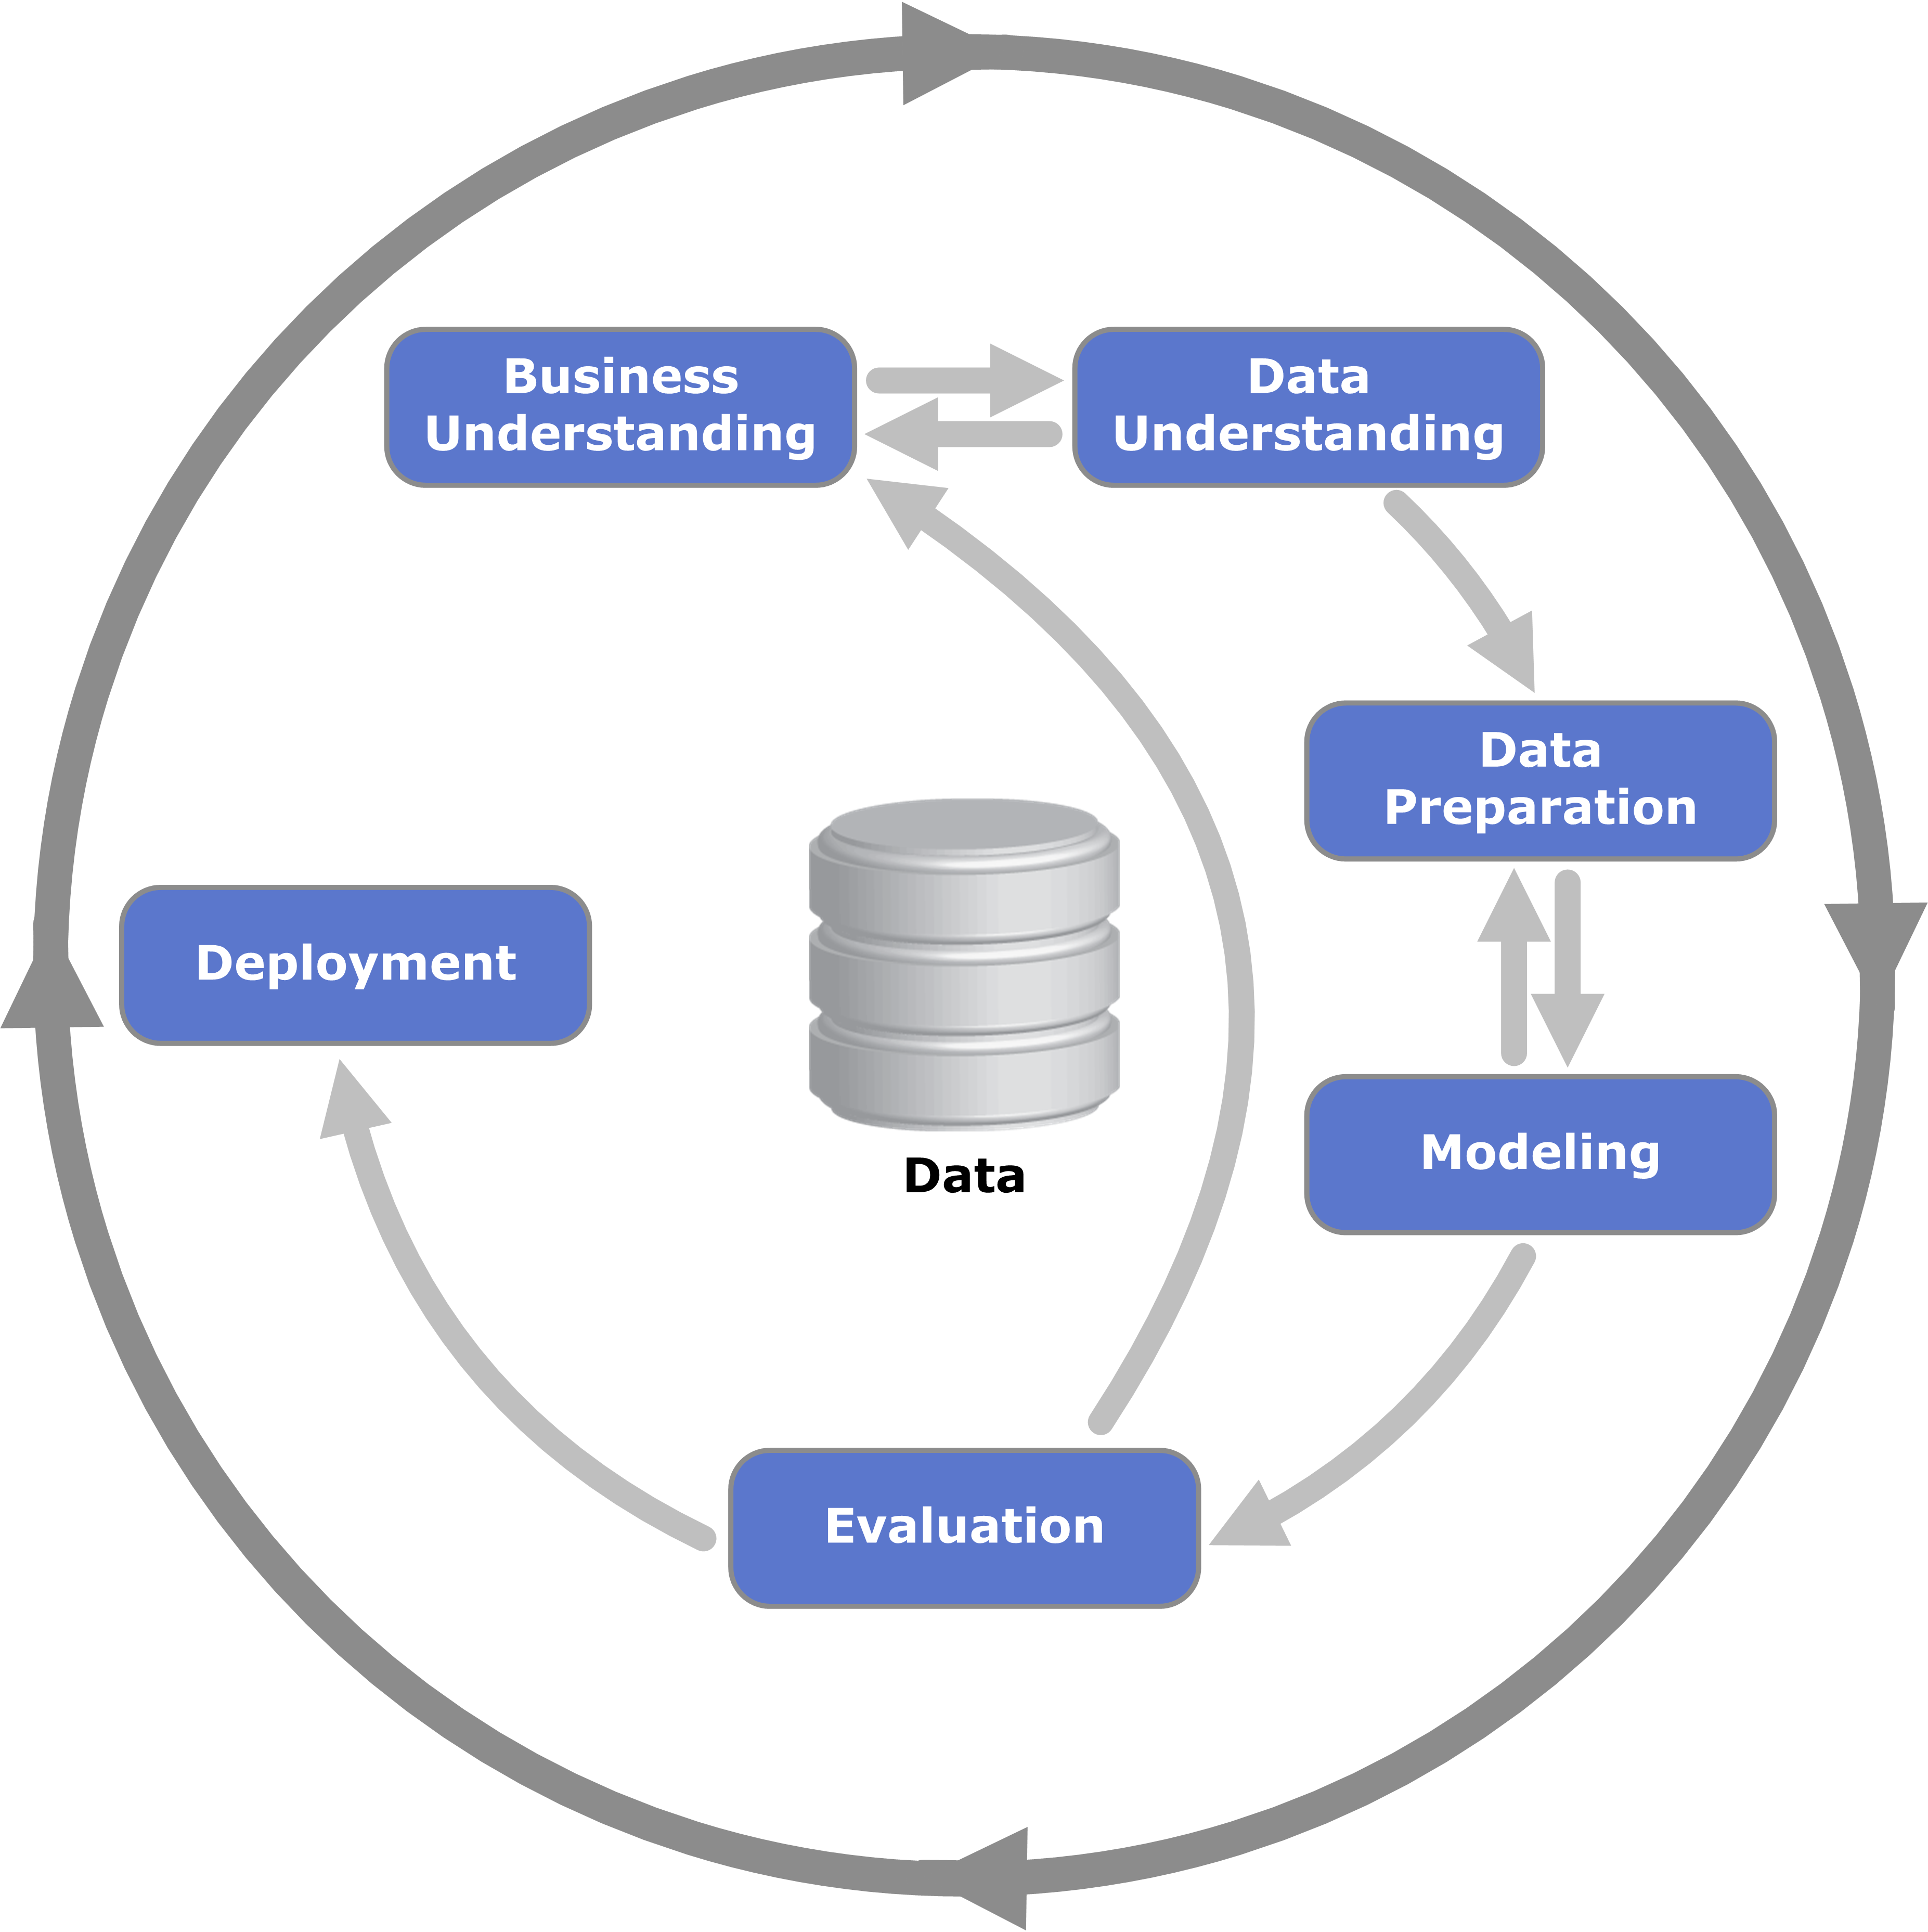
\includegraphics[width=0.65\textwidth]{crisp-dm}%
  \caption{Processo CRISP-DM}
  \label{fig:crisp-dm}
\end{figure*}

\begin{itemize}
  \item 
\textbf{Compreensão do negócio}: A compreensão do negócio ou pesquisa inclui a determinação de objetivos, a avaliação da situação atual, a definição de metas de mineração de dados e o desenvolvimento de um plano de projeto.
  \item
\textbf{Compreensão dos dados}: Uma vez que os objetivos de negócios e o plano de projeto estão estabelecidos, a compreensão dos dados considera os requisitos dos dados. Esta fase pode incluir a coleta inicial de dados, descrição dos dados, exploração dos dados e verificação da qualidade dos dados. A exploração dos dados, como a visualização sumarizada de estatísticas (que inclui a exibição visual de características categóricas) pode ocorrer no final desta fase. Métodos como análise de agrupamento também podem ser aplicados durante esta fase, com a objetivo de identificar padrões nos dados.
  \item
\textbf{Preparação dos dados}: Uma vez que os requisitos dos dados disponíveis estão identificados, eles precisam ser selecionados, limpos e estruturados na forma desejada. A limpeza de dados e a transformação de dados precisam ocorrer nessa fase. A exploração dos dados em maior profundidade pode ser aplicada durante essa fase, bem como outros métodos podem ser também utilizados, proporcionando novamente a oportunidade de identificar padrões baseados na compreensão do negócio ou pesquisa.
  \item
\textbf{Modelagem}: Após a preparação dos dados, métodos de mineração de dados (associação, agrupamento, classificação e detecção de \textit{outliers}) podem ser selecionados e aplicados. Métodos diferentes podem ser usados para o mesmo problema. Se o método resultar em um modelo, as configurações do modelo podem ser calibradas para otimizar os resultados. Esse processo pode ser repetido com novas seleções e transformações de dados, refinando gradualmente o resultado ou integrando novas fontes de dados relevantes para obter resultados diferentes, mais apropriados e valiosos.

  \item
\textbf{Avaliação}: Os resultados ou modelos devem ser avaliados conforme os objetivos de negócios definidos na fase de compreensão do negócio. Isso pode levar à identificação de outras necessidades, frequentemente retornando às fases anteriores. A obtenção de entendimento do negócio é um procedimento iterativo na mineração de dados, onde os resultados de várias ferramentas de visualização, estatística e IA mostram os novos relacionamentos que proporcionam uma compreensão mais profunda das operações organizacionais.
  \item
\textbf{Implantação}: A mineração de dados pode ser usada para validar hipóteses anteriormente realizadas ou para descoberta de conhecimento, como identificação de relacionamentos inesperados e úteis. Por meio do conhecimento encontrado nas fases anteriores do processo, os resultados ou modelos obtidos podem então serem apresentados aos \textit{stakeholders} e, então, aplicados para vários propósitos. As apresentações devem ser realizadas de forma a ajudar o \textit{stakeholder} alvo a entender, interpretar e agir sobre os resultados da mineração de dados, isso pode ser feito usando uma representação do conhecimento, como uma visualização ou relatório. Por exemplo, um analista de dados telemétricos de jogos poderia desenvolver uma visualização de \textit{heatmap} a partir dos registros de localização dos jogadores em um mapa de um jogo para apresentar ao líder de \textit{designer} do jogo, que por sua vez, poderia ter algum \textit{insight} inovador em relação ao mapa. Os resultados ou modelos precisam ser monitorados quanto as mudanças nas condições operacionais, porque o que pode ser verdade hoje pode não ser verdade no ano a partir desse instante. Se ocorrerem alterações significativas, o processo deve ser refeito. Também é aconselhável registrar os resultados dos projetos de mineração de dados, de modo que as evidências documentadas estejam disponíveis para estudos futuros.

\end{itemize}
O processo CRISP-DM em seis fases não é rígido, por meio de um procedimento exato. Geralmente, há uma grande quantidade de \textit{backtracking}. Além disso, analistas experientes podem não precisar aplicar todas as fases para um problema específico. Portanto, esse processo fornece um \textit{framework} útil para a mineração de dados.

\subsection{Preparação dos Dados}
O formato bruto dos dados geralmente é amplamente variável. Muitos valores podem estar faltando, inconsistentes em diferentes fontes de dados e errôneos. Para o analista, isso leva a inúmeros desafios na utilização eficiente dos dados. Por exemplo, considere o caso de avaliar os interesses dos consumidores a partir de suas atividades em um site de redes sociais. O analista pode primeiro determinar os tipos de atividades que são valiosos para o processo de mineração. A atividade pode corresponder aos interesses inseridos pelo usuário, aos comentários inseridos pelo usuário e ao conjunto de amizades do usuário junto com seus interesses. Todas essas informações são diversas e precisam ser coletadas de diferentes bancos de dados no site de redes sociais. Além disso, algumas formas de dados, como \textit{logs} brutos, muitas vezes não podem ser diretamente usados devido à sua natureza não estruturada. Em outras palavras, características importantes precisam ser extraídas dessas fontes de dados. Por isso existe a necessidade da fase de preparação dos dados.

A fase de preparação de dados é um processo de vários estágios que compreendem várias etapas individuais, algumas ou todas podem ser usadas em uma determinada aplicação. Essas etapas são as seguintes:

\begin{itemize}
  \item
\textbf{Extração de Características}: Dados brutos geralmente estão em uma forma que não é adequada para o processamento. Os exemplos incluem \textit{logs} brutos, documentos, dados semiestruturados e possivelmente outras formas de dados heterogêneos. Nesses casos, pode ser desejável obter características significativas a partir dos dados. Geralmente, as características com boa interpretação semântica são mais desejáveis porque simplificam a capacidade do analista de entender os resultados intermediários e geralmente têm melhor ligação aos objetivos da aplicação de mineração de dados. Em alguns casos onde os dados são obtidos de múltiplas fontes, os dados precisam ser integrados em uma única base de dados para serem processados. Além disso, alguns algoritmos podem funcionar apenas com um tipo de dados específico, sendo que os dados podem conter tipos heterogêneos. Nesses casos, a portabilidade dos tipos de dados se torna importante quando os atributos de um tipo são transformados em outro. Isso resulta em um conjunto de dados mais homogêneo que pode ser processado pelos algoritmos existentes.
  \item
\textbf{Limpeza de dados:} Na fase de limpeza de dados, os itens faltantes, errados e inconsistentes são removidas dos dados. Alguns itens faltantes também podem ser estimadas para serem inseridos nos dados.
  \item
\textbf{Redução e transformação de dados}: Nessa fase, o tamanho dos dados é reduzido através da seleção de subconjuntos de dados, seleção de subconjuntos de características ou transformação de dados. Os ganhos obtidos nesta fase são duplos. Primeiro, quando o tamanho dos dados é reduzido, os algoritmos geralmente são mais eficientes. Em segundo lugar, se características irrelevantes ou itens irrelevantes são removidos, a qualidade do processo de mineração de dados é melhorada. O primeiro objetivo pode ser alcançado por técnicas genéricas de amostragem ou redução de dimensionalidade. Para alcançar o segundo objetivo, uma abordagem altamente específica do problema em questão deve ser usada para seleção de características. Por exemplo, uma abordagem de seleção de características que funciona bem para agrupamento pode não funcionar bem para classificação.
\end{itemize}

\subsection{Extração de Características}
A primeira fase de extração de características é crucial, embora seja muito específica para a aplicação. Em alguns casos, a extração de características está intimamente relacionada ao conceito de portabilidade de tipo de dados, onde características de baixo nível de um tipo podem ser transformados em características de nível superior de outro tipo. A natureza da extração de características depende do domínio do qual os dados são coletados.

A extração de características é uma forma de arte que é altamente dependente da habilidade do analista em escolher as características e a representação que melhor se adequam ao problema. Embora este aspecto específico da análise de dados geralmente pertença ao especialista do domínio, talvez isso seja o mais importante. Se as características corretas não forem extraídas, a análise só pode ser tão boa quanto os dados disponíveis.

\subsubsection{Limpeza de Dados}
O processo de limpeza de dados é importante por causa de erros associados ao processo de coleta de dados. Problemas de qualidade em dados brutos podem vir de várias formas, por exemplo, erros ortográficos durante a entrada de dados, informações faltantes ou presença de dados inválidos. Quando várias fontes de dados são integradas em uma base de dados ou uma análise  é realizada usando múltiplas fontes de dados (por exemplo, telemetria de diferentes jogos), uma limpeza de dados mais cuidadosa  deve ser realizada devido ao potencial de erro introduzido quando os conjuntos de dados são combinados \cite{el2016game}.

Os problemas mencionados acima podem ser uma fonte significativa de imprecisão para aplicações de mineração de dados. São necessários métodos para remover ou corrigir itens faltantes e incorretos dos dados. Existem, portanto, diversos aspectos importantes da limpeza de dados:

\begin{itemize}
  \item
\textbf{Tratamento de entradas faltantes}: Muitos itens nos dados podem permanecer não especificados por causa de deficiências na coleta de dados ou na natureza inerente dos dados. Esses itens faltantes podem precisar ser estimados. O processo de estimativa de itens faltantes também é chamado de imputação.
  \item
\textbf{Tratamento de entradas incorretas}: Nos casos em que um mesmo dado está disponível em várias fontes, podem ser detectadas inconsistências. Tais inconsistências podem ser removidas como parte do processo analítico. Outro método para detectar as entradas incorretas é usar o conhecimento específico do domínio sobre o que já se sabe sobre os dados. Por exemplo, se a altura de uma pessoa for listada como 6 metros, provavelmente está incorreta. De modo mais geral, os pontos de dados que são incompatíveis com a distribuição de dados restante são frequentemente ruidosos. Esses pontos de dados são referidos como \textit{outliers}. No entanto, é perigoso assumir que esses pontos de dados são sempre causados por erros.
\end{itemize}

\subsubsection{Redução e Transformação de Dados}
O objetivo da redução de dados é representar os dados de forma mais compacta. Quando o tamanho dos dados é menor, é mais fácil aplicar algoritmos sofisticados e computacionalmente custosos. A redução dos dados pode ser em termos do número de linhas (entradas, registros ou itens) ou em termos de número de colunas (dimensões). A redução de dados resulta em alguma perda de informação. O uso de um algoritmo mais sofisticado às vezes pode compensar a perda de informações resultante da redução de dados. Diferentes tipos de redução de dados são usados em várias aplicações:

\begin{itemize}
  \item 
\textbf{Amostragem de dados}: Os registros de dados são amostrados para criar uma base de dados muito menor. A amostragem geralmente é mais difícil no cenário de fluxo de dados (\textit{streaming}) onde a amostra precisa ser mantida dinamicamente.
  \item 
\textbf{Seleção de Características}: Somente um subconjunto de características dos dados é usado no processo analítico. Normalmente, esses subconjuntos são escolhidos de uma maneira específica de aplicação. Por exemplo, um método de seleção de características que funciona bem para análise de agrupamentos pode não funcionar bem para a classificação e vice-versa.
  \item 
\textbf{Redução de dados pela rotação de eixo}: As correlações dos dados são aprimoradas para representar os dados em um número menor de dimensões. Um exemplo desse método de redução de dados inclui a análise de componente principal (\textit{Principal Component Analysis }- PCA).
  \item 
\textbf{Redução de dados pela transformação de tipo}: Esta forma de redução de dados está intimamente relacionada à portabilidade de tipo de dados. Por exemplo, séries temporais são convertidas em dados multidimensionais de tamanho ou complexidade menores usando transformações de discretização. Da mesma forma, grafos podem ser convertidos também em representações multidimensionais.
\end{itemize}

Na etapa de transformação de dados, os dados podem ser transformados ou consolidados em formas apropriadas para mineração. Estratégias para a transformação de dados incluem os seguintes:

\begin{itemize}
  \item 
  \textbf{Suavização}: A suavização é usada para remover o ruído dos dados. Alguns métodos incluem \textit{binning} \footnote{\textit{Binning} é uma maneira de agrupar uma série de valores mais ou menos contínuos em um número menor de "caixas".}, regressão e agrupamento.
  \item
\textbf{Agregação}: Métodos de sumarização ou agregação são aplicadas aos dados. Por exemplo, os dados diários de tiros de um jogador podem ser agregados de modo a calcular quantidades mensais e anuais totais. Esse passo geralmente é usado para  construção características básicas a partir de atributos.
  \item 
\textbf{Normalização}: Os dados são dimensionadas de modo a ficar dentro de um alcance menor, como $-1$ a $1$ ou $0$ a $1$.
\end{itemize}

\subsection{Principais Tarefas de Mineração de Dados}
Em geral, tarefas de mineração de dados podem ser classificadas em duas categorias: mineração de dados descritiva e mineração de dados preditiva. O primeiro descreve um conjunto de dados de forma concisa e sumarizada e apresenta propriedades gerais interessantes dos dados; O segundo constrói um ou mais modelos para realizar inferências no conjunto de dados disponível e tenta prever o comportamento de novos conjuntos de dados.

Portanto, o modelo descritivo encontra padrões ou relacionamentos em dados e explora as propriedades dos dados examinados. Agrupamento, sumarização e análise de associação são exemplos de modelos descritivos. O agrupamento é semelhante à classificação, exceto que os grupos não estão predefinidos, mas são definidos apenas pelos dados. É um método de aprendizado não supervisionado. Corresponde a partição ou segmentação dos dados em grupos distintos de tuplas ou itens similares. Os grupos são caracterizados pelo estudo do comportamento dos dados por especialistas do domínio. O termo segmentação é usado em um contexto muito específico. A sumarização é a técnica de apresentar a informação resumida dos dados. A regra de associação encontra a associação entre os diferentes atributos. A mineração de regras de associação é um processo de dois passos: encontrar todos os conjuntos de itens frequentes, gerando regras de associação fortes a partir dos conjuntos de itens frequentes. A descoberta de sequência é um processo de encontrar os padrões de sequência nos dados. Esta sequência pode ser usada para entender uma tendência.

O modelo preditivo faz previsões sobre valores de dados desconhecidos usando valores conhecidos. Classificação, previsão e regressão são exemplos de modelos preditivos. Muitas das aplicações de mineração de dados visam prever o estado futuro dos dados. Previsão é o processo de análise dos estados atuais e passados do atributo e previsão de seu futuro estado. A classificação é uma técnica de mapeamento dos dados de destino para grupos ou classes predefinidos, isso é um aprendizado supervisionado porque as classes são predefinidas antes dos dos dados de destino serem examinados. A regressão envolve o aprendizado de uma função que mapeia o item de dados para uma variável numérica de previsão de valor real.

Uma aplicação de mineração de dados pode realizar uma ou mais das seguintes tarefas de mineração de dados:

\begin{itemize}
  \item 
\textbf{Caracterização}: É o resumo das características gerais dos objetos em uma classe alvo e produz o que é chamado de regras de característica. Os dados relevantes para uma classe específica de usuário são normalmente consultados na base de dados para serem executados através de um método de sumarização e, assim, extrair a essência dos dados em diferentes níveis de abstrações. Por exemplo, talvez seja desejável caracterizar os usuários de um jogo que regularmente jogue mais de 4 horas por dia.  
  \item 
\textbf{Discriminação}: A discriminação de dados produz o que são chamados de regras de discriminação e é basicamente a comparação das características gerais dos objetos entre duas classes referidas como classe alvo e classe contrastante. Por exemplo, pode-se comparar as características gerais dos jogadores que mais venceram partidas no último ano com aqueles que perderam. As técnicas utilizadas para a discriminação de dados são semelhantes às técnicas utilizadas para a caracterização de dados com a exceção de que os resultados de discriminação de dados incluem medidas comparativas.  
  \item 
\textbf{Análise de associação}: Análise de associação estuda a frequência de itens que ocorrem em base de dados transacionais, e com base em um limite chamado suporte, identifica os conjuntos de itens frequentes. Outro limite, a confiança, que é a probabilidade condicional do que um item, aparece em uma transação quando outro item aparece, é usado para identificar regras de associação. Isso é comumente usado para análise de cesta de mercado. Por exemplo, pode ser útil para o gerente saber quais filmes são frequentemente alugados ou se existe uma relação entre alugar um certo tipo de filmes e comprar pipoca.  
  \item 
\textbf{Classificação}: É a organização de dados em determinadas classes. A classificação usa rótulos de classe dada para ordenar os objetos na coleta de dados. As abordagens de classificação normalmente usam um conjunto de treinamento onde todos os objetos já estão associados a rótulos de classe conhecidos. O algoritmo de classificação aprende do conjunto de treinamento e gera um modelo. O modelo é usado para classificar novos objetos. Por exemplo, depois de iniciar uma política de crédito, o gerente de uma loja poderia analisar o comportamento dos clientes em relação ao seu crédito, e rotular, portanto, os clientes que receberam créditos com três possíveis rótulos "seguros", "arriscados" e "muito arriscado". A análise de classificação geraria um modelo que poderia ser usado para aceitar ou rejeitar solicitações de crédito no futuro.  
  \item 
\textbf{Previsão e regressão}: A previsão tem atraído uma atenção considerável tendo em conta as implicações potenciais da previsão bem-sucedida em um contexto de negócios. Existem dois principais tipos de previsões: pode-se tentar prever alguns valores de dados indisponíveis ou tendências pendentes, ou prever um rótulo de classe para alguns dados. O último está vinculado à classificação. Uma vez que um modelo de classificação é construído com base em um conjunto de treinamento, o rótulo de classe de um objeto pode ser previsto com base nos valores de atributos do objeto e nos valores de atributo das classes. Regressão é frequentemente referida à previsão de valores numéricos ou tendências de crescimento ou não em dados relacionados ao tempo. A principal idéia é usar um grande número de valores passados para considerar valores futuros prováveis.  
  \item 
\textbf{Análise de agrupamentos}: Semelhante à classificação, a análise de agrupamentos é a organização de dados em classes. No entanto, ao contrário da classificação, os rótulos das classes são desconhecidos e depende do algoritmo de agrupamento para descobrir classes aceitáveis. É chamado também de classificação não supervisionada, porque a classificação não é definida por determinados rótulos de classe. Existem muitas abordagens de grupo baseadas no princípio de maximizar a semelhança entre objetos em uma mesma classe (similaridade intraclasse) e minimizar a semelhança entre objetos de diferentes classes (similaridade interclasse).
  \item 
\textbf{Análise de \textit{Outliers}}: \textit{Outliers} são elementos de dados que não podem ser agrupados em uma determinada classe ou grupo. Também conhecidos como exceções ou surpresas, muitas vezes é importante que sejam identificados. Enquanto os \textit{outliers} podem ser considerados ruídos e descartáveis em algumas aplicações, eles podem revelar conhecimentos importantes em outros domínios e, portanto, podem ser muito significativos e suas análises valiosas.

\end{itemize}

\chapter{Trabalhos Relacionados}

Um conjunto de publicações tem investigado sobre MOBAs por meio de análise de dados e mineração de dados para realizar diversas tarefas.

Riolut et al. \cite{rioult2014mining} investigam como o comportamento dos jogadores em Dota 2, outro MOBA popular desenvolvido pela Valve Corporation, é relevante para prever o resultado das partidas a partir de dados posicionais dos jogadores nas partidas. Conley et al. \cite{conley2013does} e Kalyanaraman \cite{kalyanaraman2014win} apresentam, cada, um preditor de resultados de partidas e um recomendador de heróis com base em dados de composição de heróis (personagens) de equipes de Dota 2, onde cada observação corresponde a um vetor que codifica a presença ou não de um herói escolhido por um jogador na equipe. Kinkade e Lim \cite{kinkade2015dota} apresentam dois preditores de resultados de partidas de Dota 2: um preditor usa dados sumarizados do estado final das partidas e outro usa dados de composição de heróis. Ong et al. \cite{ong2015player} apresentam uma abordagem para agrupar diferentes comportamentos de desempenho individual dos jogadores e, assim, prever a equipe vencedora de uma partida com base na composição de comportamentos de jogadores das equipes. Johansson e Wikstr\"om \cite {johansson2015result} criam um modelo para prever a equipe vencedora de uma partida de Dota 2, usando dados parciais coletados à medida que uma partida avança. Schubert et al. \cite{schubert2016esports} apresentam uma técnica para segmentar dados de jogadores de Dota 2 nas partidas de maneira espacial e temporal onde cada segmento é referenciado como encontro de combate e, assim, possibilitar análises de desempenho e prever resultados de partidas com base nesses encontros.

Edge \cite{edge2013predicting} cria um modelo para prever quando os jogadores irão abandonar uma partida de Dota 2 antes de terminar, modelando o estado motivacional dos jogadores na partida. Yang et al. \cite{yang2014identifying} modelam interações entre os jogadores em partidas de Dota 2 como uma sequência de grafos para identificar padrões de combate bem-sucedidos e, assim, prever resultados de combates durante a partida. Eggert et al. \cite{eggert2015classification} apresentam uma abordagem para classificar o papel de um jogador dentro de uma equipe de Dota 2 a partir de dados sumarizados de eventos de baixo nível na partida.

Kim et al. \cite{kim2015efficiently} propõem um método baseado em dados multimodais de jogadores de LoL durante uma partida (teclado e mouse, tela do jogo, expressão facial, volume e movimento do jogador) para detectar automaticamente as vezes em que esses jogadores exibem um comportamento atípico específico, como excitação, concentração, imersão e surpresa. Cavadenti et al. \cite{cavadenti2016did} propõem um método que ajude os jogadores de Dota 2 a melhorar suas habilidades descobrindo padrões estratégicos atípicos bem-sucedidos a partir de traços comportamentais históricos, ou seja, dado um modelo que codifica uma maneira esperada de se jogar (a norma), eles investigam padrões que se desviam da norma que pode explicar o resultado de uma partida.

Shim et al. \cite{shim2014decision} propõem um esquema de suporte à decisão de jogador automático com base em dados da antiga plataforma de denúncia do LoL (O Tribunal) para encontrar jogadores com mau comportamento (tóxico), como abusos e ataques maliciosos contra outros jogadores. Kwak e Blackburn \cite{kwak2014linguistic} realizam uma série de análises linguísticas para caracterizar o comportamento linguístico de jogadores tóxicos em League of Legends usando dados de contribuição colaborativa (\textit{crowdsourcing}) de jogadores acusados como tóxicos. Blackburn e Kwak \cite{blackburn2014stfu} exploram o uso do desempenho no jogo, relatórios de vítimas de comportamentos tóxicos e características linguísticas de mensagens de jogadores tóxicos em LoL para treinar classificadores para detectar a presença e gravidade de toxicidade. Shores et al. \cite{shores2014identification} examinam a natureza e os efeitos do comportamento tóxico em League of Legends para desenvolver uma métrica chamada índice de toxicidade e investigar os efeitos da interação de outros jogadores com jogadores tóxicos, incluindo taxa de retenção de jogadores.

Pobiedina et al. \cite{pobiedina2013ranking} analisam padrões de comportamento social de trabalho em equipe usando dados de comunidades virtuais de Dota 2. Park e Kim \cite{park2014social} analisam a rede social de jogadores de LoL para encontrar conhecimento relevante que ajude, por exemplo, a entender como os jogadores formam equipes. Drachen et al. \cite{drachen2014skill} apresentam um método para investigar como o comportamento das equipes em Dota 2 varia dependendo do nível de habilidade dos jogadores, analisando seus movimentos e a distância entre eles ao longo da partida. Claypool et al. \cite{claypool2015surrender} analisam dados quantitativos e qualitativos de partidas de LoL, como duração da partida e contentamento do jogador, para investigar se partidas criadas automaticamente (\textit{matchmaking}) são equilibradas ou não. Neidhardt et al. \cite{neidhardt2015team} investigam os impactos de três categorias de fatores de equipe (habilidades dos jogadores, relações de colaboração e parcerias com jogadores em equipes anteriores) em relação ao desempenho das equipes e duração das partidas de Dota 2. Leavitt et al. \cite{leavitt2016ping} analisam jogadores em partidas de League of Legends para investigar o impacto do sistema de comunicação não-verbal (\textit{ping}) no desempenho das equipes. Buchan e Taylor \cite{buchan2016qualitative} exploram o jogo em equipe analisando as experiências subjetivas dos participantes (tais como comunicação, papel, estado psicológico e nível de habilidade de jogo) ao jogar MOBAs e, assim, criar um modelo conceitual baseado em processos de grupo tradicionais (papéis de equipe, desenvolvimento de grupo e percepções e comportamento durante o estado de desvinculação). Kim et al. \cite{kim2017makes} examinam quais fatores individuais e de grupo estão associados à inteligência colaborativa em equipes de LoL e se ela é preditiva para o desempenho dessas equipes, com base em conjuntos de dados que compreendem métricas no jogo, resultados laboratoriais e questionários de equipes.

Embora estes estudos desempenhem um papel essencial na literatura, nenhum deles se propôs a modelar perfis de equipe em LoL com base no comportamento de desempenho das equipes nas partidas, bem como, fornecer métricas de desempenho bem-sucedidas e malsucedidas de equipes que possam apoiar a tomada de decisão.

\chapter{Preparação dos Dados}
Para preparar o conjunto de dados de desempenho de equipes, foram realizadas as seguintes tarefas: coleta de dados; extração de características; limpeza de dados; remoção de características com baixa variância; detecção de \textit{outliers}; transformação de dados; normalização de dados; análise de redundância de características.

\section{Coleta de Dados}
A Riot Games, desenvolvedora do LoL, fornece uma Interface de Programação de Aplicação (\textit{Application Programming Interface} - API) baseada na Web para acessar os históricos das partidas em formato JSON \cite{riot1}. Um histórico de partida contém dados como modo de jogo \footnote{O modo clássico é o mais escolhido pelos jogadores e uma partida desse modo deve ter 10 participantes duelando uns aos outros em duas equipes diferentes.}, tipo de fila \footnote{Um jogador precisa entrar no sistema de filas para encontrar e participar de uma partida; existem vários tipos de filas em LoL}, duração da partida, time vencedor e perdedor, e número de identificação única. Um histórico contém também dados de cada jogador que participa da partida, como escolha de personagem e estatísticas sumarizadas de desempenho do jogador em toda a partida. Essas estatísticas indicam, por exemplo, dano total causado e recebido, ouro total recebido e gasto, dano total causado e sofrido, e cura total recebida na partida. A Tabela ~\ref{tab:features-desc} apresenta as descrições de todas as 37 estatísticas númericas fornecidas pela API.

\begin{table}
  \scriptsize
  \caption{Descrições das estatísticas básicas de desempenho dos jogadores em partidas.}
  \label{tab:features-desc}
  \begin{tabular}{p{0.30\textwidth}p{0.65\textwidth}}
    \toprule
    Feature & Description \\
    \midrule
assists & Número de assistências em abates\\
deaths & Número de mortes sofridas \\
doubleKills & Número de abates duplos seguidos efetuados\\
goldEarned & Quantidade de ouro ganho\\
goldSpent & Quantidade de ouro gasto\\
inhibitorKills & Número de inibidores \footnote{Inibidores são estruturas que bloqueiam a formação de \textit{Super Minions} da equipe inimiga.} destruídos\\
killingSprees & Número de matanças (abates $\geq 3$ seguidos) sem que o campeão morra \\
kills & Número de abates efetuados\\
largestCriticalStrike & Maior ataque crítico\\
largestKillingSpree & Matança com maior número de abates\\
largestMultiKill & Maior abates múltiplos seguidos\\
magicDamageDealt* & magicDamageDealtToChampions +  magicDamageDealtToMonsters\\
magicDamageDealtToChampions & Dano mágico total causado a campeões\\
magicDamageTaken & Dano mágico total recebido\\
minionsKilled & Quantidade de \textit{minions} abatidos\\
 neutralMinionsKilled* & neutralMinionsKilledEnemyJungle + neutralMinionsKilledTeamJungle\\
neutralMinionsKilledEnemyJungle & \textit{Minions} neutros abatidos na selva da equipe inimiga
\\
neutralMinionsKilledTeamJungle & \textit{Minions} neutros abatidos na selva da equipe\\
pentaKills & Número de abates quíntuplos seguidos\\
physicalDamageDealt* & physicalDamageDealtToChampions + physicalDamageDealtToMonsters\\
physicalDamageDealtToChampions & Dano físico total causado a campeões\\
physicalDamageTaken & Dano físico total recebido\\
quadraKills & Número de abates quádruplos seguidos\\
sightWardsBoughtInGame & Quantidade de itens \textit{sight wards} comprados\\
totalHeal & Quantidade de cura total efetuada\\
totalTimeCrowdControlDealt & Tempo total de controle da equipe inimiga\\
totalUnitsHealed & Total de unidades curadas\\
towerKills & Número de torres destruidas pela equipe\\
tripleKills & Número de abates triplos seguidos\\
totalDamageDealt* & physicalDamageDealt + magicDamageDealt \\
totalDamageDealtToChampions* & physicalDamageDealtToChampions + magicDamageDealtToChampions \\
 trueDamageDealt* & trueDamageDealtToChampions + trueDamageDealtToMonsters\\
trueDamageDealtToChampions & Dano verdadeiro causado a campeões\\
trueDamageTaken & Dano verdadeiro recebido\\
visionWardsBoughtInGame & Quantidade de itens \textit{vision wards} comprados\\
wardsKilled & Número de itens \textit{wards} destruidos\\
wardsPlaced & Número de itens \textit{wards} usados\\
  \bottomrule
\end{tabular}
\end{table}

Coletamos aleatoriamente da API 110.000 históricos de partidas a partir de fevereiro de 2016 até dezembro de 2016. Para cada mês, coletamos 10.000 históricos. Consideramos os seguintes filtros para a coleta: 

\begin{itemize}
  \item Região: Brasil
  \item Temporada: 2016
  \item Modo de jogo: Clássico
  \item Tipo de fila: Competitivo (\textit{ranked}) \textit{solo};
  \item Quantidade de jogadores em cada equipe: 5
  \item Versão da partida: v6.x.x
\end{itemize}

\section{Extração de Características}

% TODO
% Consider a multidimensional database D with n records, and d attributes. Such a database D may be represented as an n × d matrix D, in which each row corresponds to one record and each column corresponds to a dimension. We generally refer to this matrix as the data matrix. This book will use the notation of a data matrix D, and a database D interchangeably.

Em seguida, extraímos características das partidas coletadas para modelar nosso conjunto de dados de desempenho de equipes. Seja $M=\{m_1,...,m_{110000}\}$ um conjunto de histórico de partidas, $T=\{t_1, ..., t_n | n=110000 * 2=220000\}$ um conjunto de equipes, $P=\{p_1, ..., p_{|P|}\}$ um conjunto dimensional $d=38$ de estatísticas básicas de desempenho dos jogadores nas partidas. Uma partida consiste de duas equipes distintas $m=\{t_a,t_b\}$ e uma equipe é composta pelo desempenho de 5 jogadores distintos $t=\{p_k |  p_k \in P^t; P^t \supset P; 1 \geq k \leq 5\}$. Selecionamos as estatísticas de desempenho dos jogadores nas partidas e somamos cada estatística $P_j \in P$ por equipe para formar cada característica (ou estatística) $X_j \in X_{220000, 38}$ do nosso conjunto de desempenho de equipes, de modo que $X = \{ x_{i} = \sum_{k=1}^{5} p_{k}^{i} | t_{i} \in T; p_{k}^{i} \in P \}$.

Finalmente, para garantir a atomicidade no conjunto de dados $X$, decompomos algumas características, por exemplo, subtraimos \textit{physicalDamageDealt} de \textit{physicalDamageDealtToChampions} para computar \textit{physicalDamageDealtToMonsters} e subtraímos \textit{magicDamageDealt} de \textit{magicDamageDealtToChampions} para computar \textit{magicDamageDealtToMonsters}. Para evitar redundância nos dados, removemos também características compostas, por exemplo, características que são soma de outras:

\begin{itemize}
  \item \textit{totalDamageDealt = physicalDamageDealt + magicDamageDealt}
  \item \textit{totalDamageDealtToChampions = physicalDamageDealtToChampions + magicDamageDealtToChampions}
  \item \textit{totalDamageTaken = physicalDamageTaken + magicDamageTaken}
  \item \textit{neutralMinionsKilled = neutralMinionsKilledEnemyJungle + neutralMinionsKilledTeamJungle}
  \item \textit{trueDamageDealt = trueDamageDealtToChampions + trueDamageDealtToMonsters}
  \item \textit{physicalDamageDealt = physicalDamageDealtToChampions + physicalDamageDealtToMonsters}
  \item \textit{magicDamageDealt = magicDamageDealtToChampions + magicDamageDealtToMonsters}
\end{itemize}

A Tabela ~\ref{tab:features-desc} indica com (*) as características compostas removidas.

\section{Limpeza de Dados}
Para evitar conclusões falsas, realizamos a limpeza de dados para detectar e remover inconsistências no conjunto de desempenho das equipes. Em nossa análise, removemos partidas com as seguintes condições:

\begin{itemize}
\item Partidas rendidas: dependendo se uma partida está extremamente desequilibrada, geralmente a equipe que está perdendo pode solicitar a rendição a equipe inimiga a qualquer momento após 20 minutos do início da partida.
\item Partidas que contêm jogadores que abandonam: Como as partidas de LoL são jogadas \textit{online}, os jogadores podem sair das partidas a qualquer momento. Alguns motivos incluem perda de conexão, desistência ou outro motivo desconhecido. Esses abandonos podem causar também um desequilíbrio nas partidas.
\end{itemize}

\section{Remoção de Características com Baixa Variância}
Às vezes, os valores de algumas características têm variância zero ou próxima de zero, o que implica que essas características são também não informativas e podem causar ruído ao executar uma determinada tarefa de mineração de dados. Portanto, realizamos uma estatística descritiva no conjunto de dados para identificar e remover características de variância zero ou próxima de zero. Após a análise, o conjunto de dados foi reduzido. As seguintes características foram removidas: \textit{doubleKills}, \textit{inhibitorKills}, \textit {largestMultiKill}, \textit{pentaKills}, \textit {quadraKills}, \textit {sightWardsBoughtInGame} e \textit{tripleKills}.

\section{Detecção de Outliers}
Utilizamos um Intervalo Interquartil de $fator = 1,5$ para encontrar valores anômalos em cada característica no conjunto de dados. Equipes com alguma característica anômala foram removidas dos dados. Em seguida, realizamos uma análise para remover características com baixa variância novamente. Após a análise, as seguintes características foram removidas: \textit{totalUnitsHelead} e \textit{visionWardsBoughtInGame}.

\section{Transformação de Dados}
O conjunto de dados $X$ é apenas um reflexo do desempenho das equipes durante a partida, ou seja, estatísticas sumarizadas. Como a duração de uma partida não tem limite de tempo, é necessário transformar os dados para tornar o desempenho das equipes comparáveis entre si, independentemente da duração das partidas. Assim, para lidar com o problema de capturar o desempenho das equipes em diferentes durações de partidas, calculamos a divisão de desempenho de cada equipe $x \in X$ pela duração $duration$ da partida $m$ em que a equipe participou:

\begin{displaymath}
  \frac{x}{m^{duration}}
\end{displaymath}

Dessa forma, como discutimos na seção 2.2.1, as características do nosso conjunto de dados deixam de ser simples estatísticas básicas para se tornarem métricas de desempenho. Por exemplo, as características agora passam a ser número de assistências em abates por minuto (\textit{assists}), número de mortes sofridas por minuto (\textit{deaths}), número de abates duplos seguidos efetuados por minuto (\textit{doubleKills}), e assim por diante.

\section{Normalização de Dados}
Realizamos uma análise de \textit{boxplot} no conjunto de dados transformados e descobrimos que o intervalo de valores varia amplamente entre as características. Portanto, aplicamos a normalização de de dados \cite{zaki2014data} nas características para que cada uma contribua proporcionalmente em uma mesma escala na realização da análise de redundância e agrupamento. Seja $X$ um conjunto de dados e $x_1, ..., x_n $ uma amostra aleatória retirada de $X$, aplicamos a normalização baseada nos valores \textit{mínimo} e \textit{máximo} para escalar a característica pelo intervalo $r$ da amostra de $X$:

\begin{displaymath}
  x'=\frac{x_i - min(X)}{r}=\frac{x_i - min(X)}{max(X)-min(X)}
\end{displaymath}

Após a normalização, o conjunto de dados $X$ assumiu valores na faixa $[0, 1]$.

\section{Análise de Redundância}

Para identificar e remover característica redundantes no conjunto de dados, realizamos uma análise de correlação. Com base no teste de correlação de Spearman \cite{xiao2015using}, consideramos que um par de características de alta ou altíssima correlação são redundantes. A Figura ~\ref{fig:correlations} ilustra o gráfico de correlação entre as $d=24$ características do conjunto de dados $X$. De acordo com o gráfico, podemos observar que existem várias características redundantes.

\begin{figure*}
  \centering
  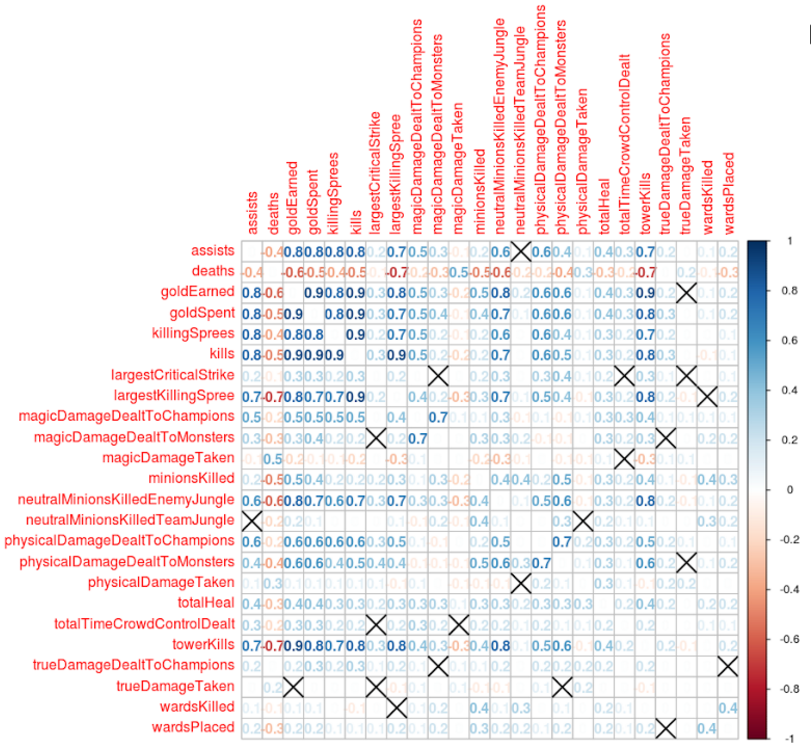
\includegraphics[width=1.0\textwidth]{correlations}%
  \caption{Gráfico de correlação para as características de desempenho das equipes.}
  \label{fig:correlations}
\end{figure*}

Desse modo, para cada par de características $(X_a, X_b); a, b=\{1, ..., d\};a \neq b$ com alta ou altíssima correlação $r_{ab} >= 0.65$, removemos de $X$ a característica que tem a maior correlação no par, ou seja, a característica do par em que a soma de todas as suas correlações com as demais características de $X$ tem o maior valor:

\begin{displaymath}
  max \big\{ \sum_{i=1}^{d} r_{ai} ,  \sum_{i=1}^{d} r_{bi} \big\}; a \neq i; b \neq i
\end{displaymath}

Portanto, removemos as seguintes características: \textit{assists}; \textit{goldEarned}; \textit{goldSpent}; \textit{kills}; \textit{largestKillingSpree}; \textit{magicDamageDealtToChampions}; \textit{physicalDamageDealtToChampions}; \textit{towerKills}.

\chapter{Agrupamento de Dados}

O problema de encontrar perfis de equipe é equivalente ao problema de identificar um conjunto de grupos de equipes de comportamento semelhante. Para abordar esse problema, usamos o método de mineração de dados \textit{K-means clustering} \cite{zaki2014data}. Dado um conjunto dimensional de observações \(x_1, ..., x_n \), o \textit{K-means clustering} visa particionar as $n$ observações em $k (\leq n)$ grupos distintos, denotados por $ C = \{c_1, ... , c_k \} $, de modo a minimizar a Soma dos Quadrados do Erro Dentro dos Grupos (SQED); ou seja, seu objetivo é encontrar o minimizador $C*$ da função da Soma dos Quadrados do Erro (SQE):

\begin{displaymath}
  SQE(C) = \sum_{i=1}^{k} \sum_{x_j \in c_i}{} || x_j - \mu _i ||^2
\end{displaymath}

Onde $\mu_j$ é a média das observações em $c_i$, e indica também o \textit{i}-ésimo centróide de $C$.

Conforme Zaki et al. \cite{zaki2014data}, o \textit{K-means} usa uma abordagem iterativa gananciosa (\textit{iterative greedy}) para encontrar um grupo que minimize a função objetivo $SSE$ e, como tal, pode convergir para um grupo ótimo local em vez de um grupo ótimo global.

Em nosso conjunto de dados $X$ usamos o algoritmo de Lloyd \cite{ong2015player}, uma heurística que consiste em escolher aleatoriamente observações como centróides para os $k$ grupos de $C$ e atribuir iterativamente cada observação $x \in X$ ao centróide mais próximo e depois atualizar os centróides com a média de seus respectivos grupos.

Para encontrar um número ótimo $k$ de grupos usamos um método que encontra o "\textit{joelho}"  da curva de erro. Este método tenta descobrir um número apropriado de grupos analisando a curva de um gráfico gerado a partir de um teste realizado para cada número possível de grupos \cite{salvador2004determining}. No nosso caso, o teste foi baseado na função objetivo $SQE$.

A Figura ~\ref{fig:k-means-curve} ilustra o gráfico SQE para cada número possível de grupos $K = \{1, ..., 120\}$. Como podemos observar, o conjunto de dados $X$ pode ser particionado em $k=7$ grupos distintos. Ao atribuir cada $x \in X$ em um grupo $c \in C$, conseguimos diminuir a variabilidade dos dados em aproximadamente $78\%$, ou seja, obtivemos uma proporção entre a Soma dos Quadrados do Erro Entre os Grupos (SQEE) e a Soma dos Quadrados do Erro Total (SQET) de $SQEE/SQET = 78 \%$.

\begin{figure*}
  \centering
  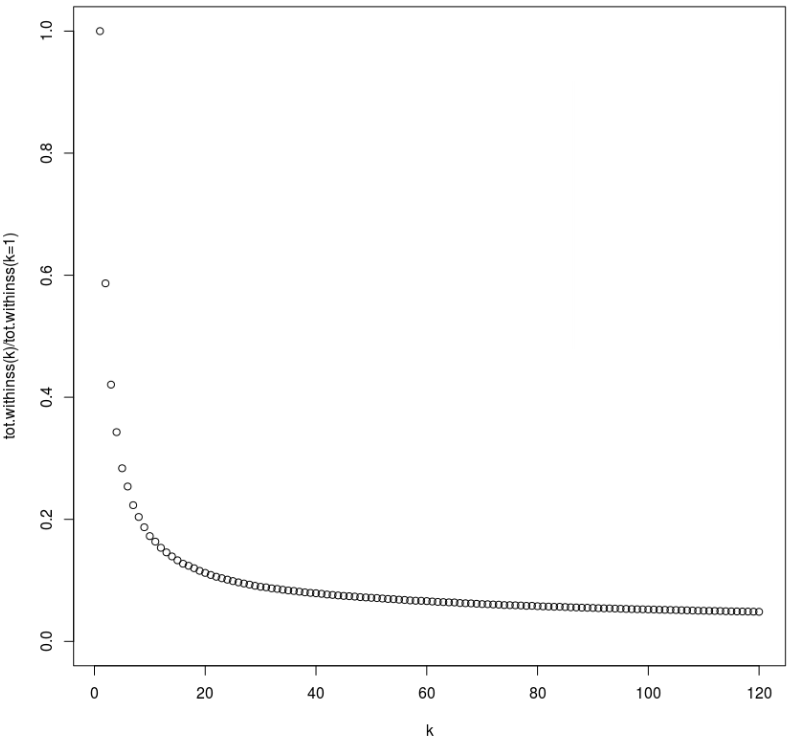
\includegraphics[width=1.0\textwidth]{k-means-curve}%
  \caption{K-means SSE curve: $BBSSE(k)/TSSE$   for each  $k \in {1:120}$}
  \label{fig:k-means-curve}
\end{figure*}

\chapter{Caracterização de perfis}
Neste capítulo, caracterizamos e definimos rótulos para os grupos de conjunto de desempenho de equipes de modo a colocar em perspectiva suas principais características ou estatísticas de desempenho. A fim de compreender como os grupos encontrados se diferem entre si, analisamos:

\begin{enumerate}[label=(\roman*)]
 \item A quantidade de equipes e a taxa de equipes vencedoras/perdedoras;
 \item Os centróides que sumarizam as características dos grupos;
 \item Em que medida as características têm influência ou relevância nos grupos.
\end{enumerate}

A Figura ~\ref{fig:win-table} e a Figura ~\ref{fig:win-plot} ilustram como os grupos diferem entre si em termos de quantidade de equipes e taxa de equipes vencedoras/derrotadas.

A Figura ~\ref{fig:relevance} ilustra o mapa de calor da análise de relevância das características com base no cálculo do ganho de informação aplicado ao conjunto de métricas desempenho das equipes sem normalização (realizado na seção 4.7) $M$ para indicar como eles influenciam cada grupo.

Seja $A$ a matriz de centróides dos grupos das métricas de desempenho das equipes $M$, cada linha $a \in A$ indica os centróides das características de um grupo, e cada coluna $A_j \in A$ indica os centróides de uma determinada característica através dos grupos. A Tabela ~\ref{tab:centers} apresenta o conjunto transposto dos centróides $t(A)$ e denota como eles se diferem em termos de desempenho.

A Figura ~\ref{fig:radars} ilustra os gráficos de radar dos grupos, onde cada gráfico de radar representa as métricas de desempenho de um grupo, cada eixo representa uma métrica de desempenho e o comprimento do eixo indica qual a pontuação do grupo em uma métrica de desempenho específica. As métricas de desempenho usadas para modelar os gráficos de radar são baseadas nos centróides dos grupos normalizados por característica $normalization(A_j)$, de modo que o comprimento de um eixo seja proporcional em todos os centróides dos grupos e assuma um valor entre [0, 1].

Ao observar os resultados, dividimos os grupos em quatro níveis em termos de taxa de equipes vencedoras: muito baixo, moderado, alto e muito alto. Nos parágrafos seguintes, elaboramos esses resultados ao caracterizar os grupos de desempenho das equipes para cada nível de taxa de equipes vencedoras.

\begin{figure*}
  \centering
  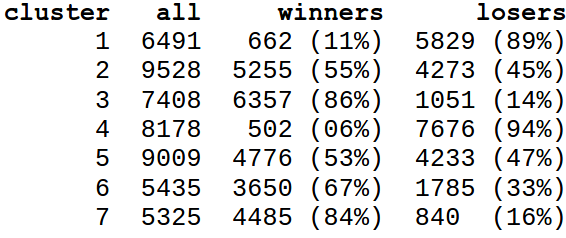
\includegraphics[width=0.5\textwidth]{win-rate-table}%
  \caption{Distribuição da quantidade de equipes vencedoras (\textit{winners}) e perdedoras (\textit{losers}).}
  \label{fig:win-table}
\end{figure*}

\begin{figure*}
  \centering
  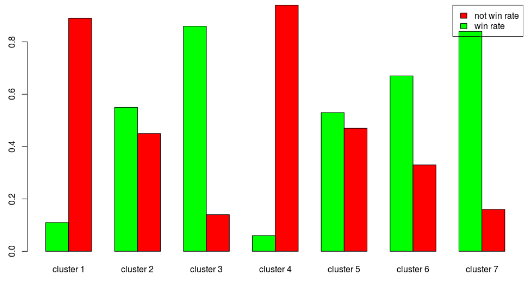
\includegraphics[width=0.7\textwidth]{win-rate-plot}%
  \caption{Gráfico de barras das taxas de equipes vencedoras (\textit{win rate}) e perdedoras (\textit{not win rate}) dos grupos.}
  \label{fig:win-plot}
\end{figure*}

\begin{figure*}
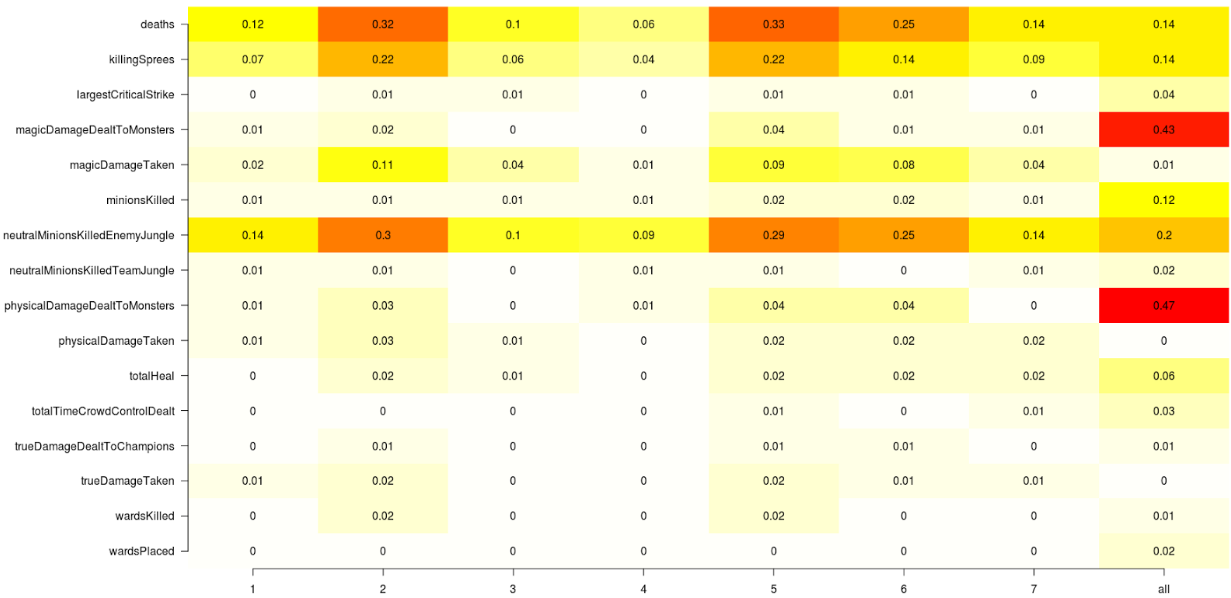
\includegraphics[width=1\textwidth,height=\textheight,keepaspectratio]{relevance}
\caption{Mapa de calor das relevâncias das métricas desempenho das equipes com base no ganho de informação.}
\label{fig:relevance}
\end{figure*}

\begin{table*}
  \tiny
  \caption{Centroides das características (métricas) para cada cluster. O mínimo e o máximo são indicados por linha}
  \label{tab:centers}
  \begin{tabular}{lp{0.08\textwidth}p{0.07\textwidth}p{0.08\textwidth}p{0.08\textwidth}p{0.08\textwidth}p{0.08\textwidth}p{0.09\textwidth}p{0.05\textwidth}}
  \toprule
Característica&                   Grupo 1&      Grupo 2&      Grupo 3&      Grupo 4&      Grupo 5&      Grupo 6&        Grupo 7&     Todos\\
  \midrule
deaths&                             1.17&    0.85&    $0.73^{min}$&    $1.22^{max}$&    0.87&    0.79&     0.74&    0.92\\ \hline
killingSprees&                      0.14&    0.22&    $0.26^{max}$&    $0.12^{min}$&    0.22&    0.23&     $0.26^{max}$&    0.21\\ \hline
largestCriticalStrike&             $22.85^{min}$&   31.63&   40.80&   26.11&   35.52&   30.65&    $46.64^{max}$&   33.10\\ \hline
magicDamageDealtToMonsters&      4805.31& 5077.61& 5621.34& $2662.17^{min}$& 3043.93& $7716.26^{max}$&  3174.08& 4462.33\\ \hline
magicDamageTaken&                1187.75& 1118.98& $1108.49^{min}$& 1157.09& $1095.07^{max}$& 1145.94&  1087.15& 1127.58\\ \hline
minionsKilled&                     15.55&   17.73&   19.39&   $15.03^{min}$&   17.57&   18.69&    $19.45^{max}$&   17.52\\ \hline
neutralMinionsKilledEnemyJungle&    0.20&    0.48&    0.77&    $0.18^{min}$&    0.49&    0.58&     $0.81^{max}$&    0.48\\ \hline
neutralMinionsKilledTeamJungle&     1.93&    2.10&    2.33&    $1.87^{min}$&    2.10&    2.24&     $2.33^{max}$&    2.12\\ \hline
physicalDamageDealtToMonsters&   $4661.69^{min}$& 7414.61& 9875.30& 6138.25& 9103.80& 6361.48& $12198.87^{max}$& 7899.13\\ \hline
physicalDamageTaken&             1986.43& 2014.44& 2066.65& $1979.37^{min}$& 2026.98& 2029.57&  $2083.44^{max}$& 2023.80\\ \hline
totalHeal&                        489.48&  603.20&  $694.18^{max}$&  $440.94^{min}$&  580.17&  685.86&   671.94&  587.95\\ \hline
totalTimeCrowdControlDealt&        51.15&   58.48&   $62.06^{max}$&   $46.86^{min}$&   53.69&   64.16&    56.57&   55.78\\ \hline
trueDamageDealtToChampions&        $85.38^{min}$&  100.79&  107.55&   90.51&  110.61&   95.45&   $116.25^{max}$&  100.94\\ \hline
trueDamageTaken&                  $109.38^{(max)}$&  $103.26^{min}$&  105.52&  106.13&  101.85&  105.99&   105.82&  105.12\\ \hline
wardsKilled&                        0.20&    0.23&    $0.27^{max}$&    $0.17^{min}$&    0.21&    $0.27^{max}$&     0.25&    0.23\\ \hline
wardsPlaced&                        1.62&    1.76&    $1.85^{max}$&    $1.56^{min}$&    1.73&    1.83&     1.82&    1.73\\
  \bottomrule
\end{tabular}
\end{table*}

\begin{figure*}
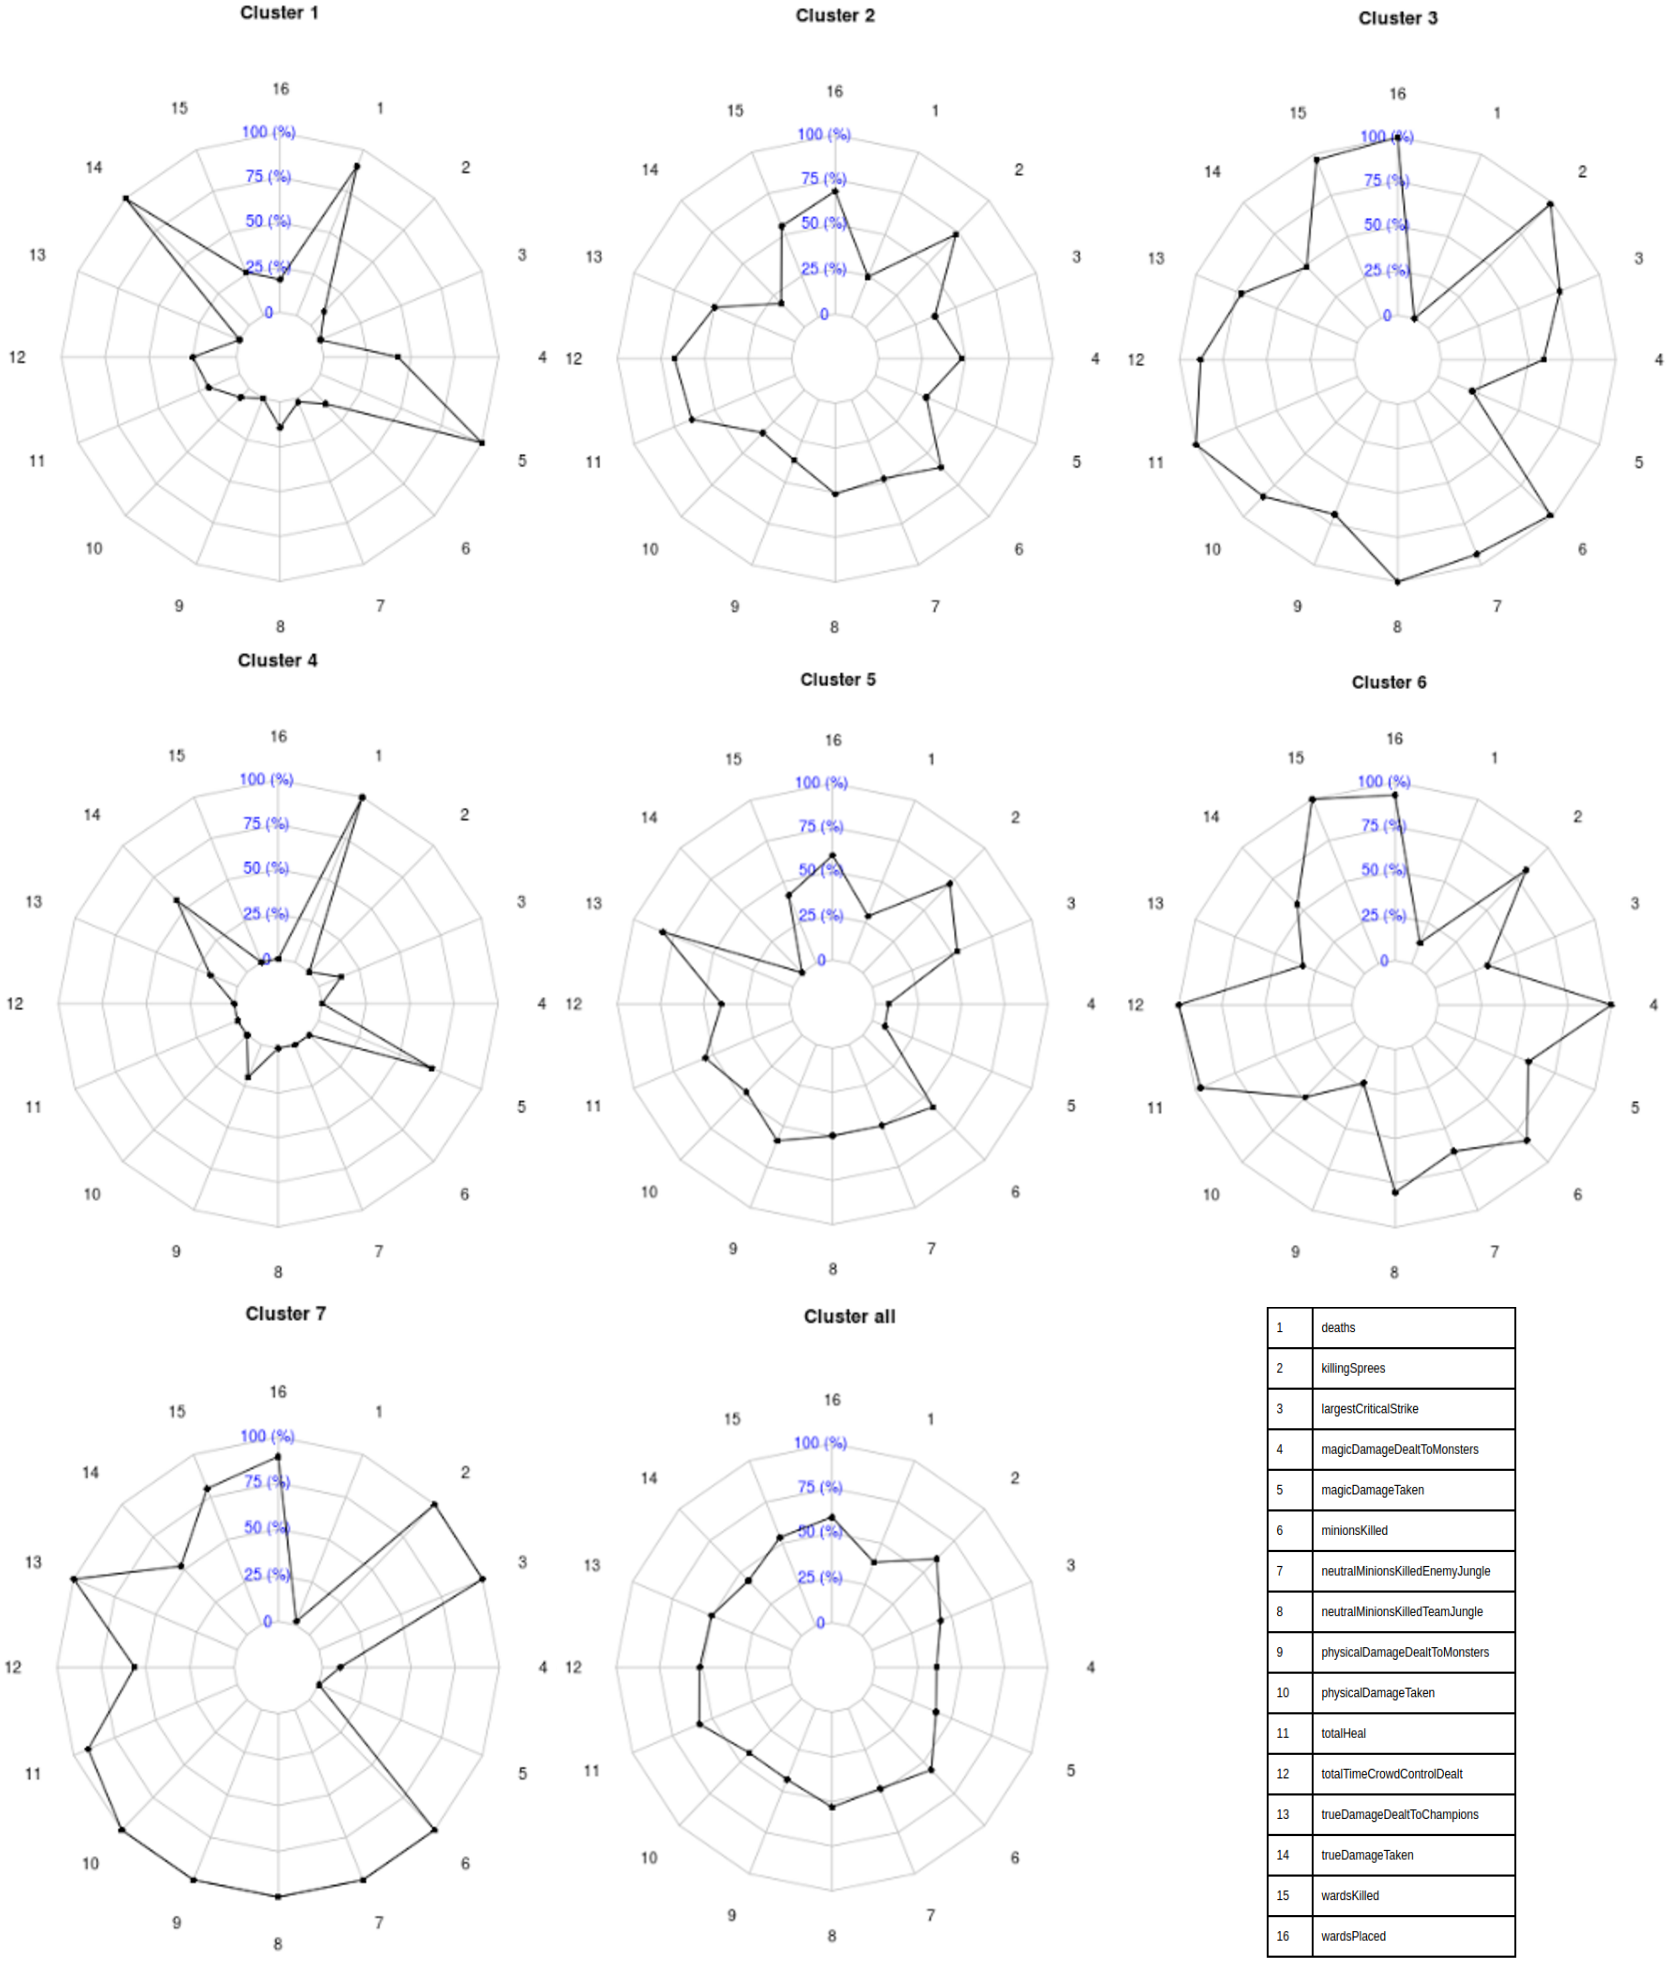
\includegraphics[width=1\textwidth,height=\textheight,keepaspectratio]{radars}
\caption{Centróides dos grupos normalizados por métrica de desempenho das equipes.}
\label{fig:radars}
\end{figure*}

\section{Nível Muito Baixo}
O nível de desempenho muito baixo consiste do \textit{Grupo 1} e \textit{Grupo 4}. Esse nível é distinguido por uma taxa de equipes vencedoras muito baixa $w_r = 10 \%$ e uma taxa de equipes perdedoras muito alta $l_r = 90 \%$ (Figura ~\ref{fig:win-plot}, Figura ~\ref{fig:win-table}). Existem 10 características relevantes para o \textit{Grupo 1} e 7 características relevantes para o \textit{Grupo 4} (Figura ~\ref{fig:relevance}). Os mais relevantes ordenados por importância são: \textit{neutralMinionsKilledEnemyJungle}, \textit{deaths}, \textit{killingSprees}. A Tabela ~\ref{tab:clusters-very-low} resume as semelhanças e diferenças entre as pontuações das métricas de desempenho para os grupos desse nível (Figura ~\ref{fig:radars}). As pontuações que mais se diferenciam entre os grupos são: \textit{magicDamageDealtToMonsters} (moderado para o \textit{Grupo 1} e muito baixo para o \textit{Grupo 4}) e \textit{trueDamageTaken} (muito alto para o \textit{Grupo 1} e o moderado para o \textit{Grupo 4}).

\begin{table}
  \scriptsize
  \caption{Nível das pontuações de desempenho para o Grupo 1 e Grupo 4.}
  \label{tab:clusters-very-low}
  \begin{tabular}{p{0.1\textwidth}p{0.265\textwidth}p{0.265\textwidth}p{0.265\textwidth}}
    \toprule
    \textbf{Score level} & \textbf{Grupo 1 e Grupo 4} & \textbf{Grupo 1} & \textbf{Grupo 4} \\
    \midrule
Very low & killingSprees (2), largestCriticalStrike (3), minionsKilled (6), neutralMinionsKilledEnemyJungle (7), neutralMinionsKilledTeamJungle (8), physicalDamageTaken (10) & physicalDamageDealtToMonsters (9), trueDamageDealtToChampions (13) & magicDamageDealtToMonsters (4), totalHeal (11), totalTimeCrowdControlDealt (12), wardsKilled (15), wardsPlaced (16) \\
    \hline
Low & & totalHeal (11), totalTimeCrowdControlDealt (12), wardsKilled (15), wardsPlaced (16) & physicalDamageDealtToMonsters (9), trueDamageDealtToChampions (13) \\
    \hline
Middle & & magicDamageDealtToMonsters (4) & trueDamageTaken (14) \\
    \hline
High & & & magicDamageTaken (5) \\
    \hline
Very High & deaths (1) & magicDamageTaken (5), trueDamageTaken (14) & \\
  \bottomrule
\end{tabular}
\end{table}

\section{Nível Moderado}
O nível de desempenho moderado consiste dos \textit{Grupo 2} e \textit{Grupo 5}. Esse nível é distinguido por uma taxa de equipes vencedoras moderada $w_r = 55 \%$ e uma taxa de equipes perdedoras baixa $l_r = 45 \%$ (Figura ~\ref{fig:win-plot}, Figura ~\ref{fig:win-table}). Existem 14 características relevantes para o \textit{Grupo 2} e 15 características relevantes para o \textit{Grupo 5} (Figura ~\ref{fig:relevance}). Os mais relevantes ordenados por importância são: \textit{deaths}, \textit{neutralMinionsKilledEnemyJungle}, \textit{killingSprees}, \textit{magicDamageTaken}. A Tabela ~\ref{tab:clusters-moderate} resume as semelhanças e diferenças entre as pontuações das métricas de desempenho para os grupos desse nível (Figura ~\ref{fig:radars}). A pontuação que mais se diferencia entre os grupos é: \textit{magicDamageDealtToMonsters} (moderado para o \textit{Grupo 2} e muito baixo para o \textit{Grupo 5}).

\begin{table}
  \scriptsize
  \caption{Nível das pontuações de desempenho para o Grupo 2 e Grupo 5.}
  \label{tab:clusters-moderate}
  \begin{tabular}{p{0.1\textwidth}p{0.265\textwidth}p{0.265\textwidth}p{0.265\textwidth}}
    \toprule
    \textbf{Score level} & \textbf{Grupo 2 e Grupo 5} & \textbf{Grupo 2} & \textbf{Grupo 5} \\
    \midrule
Very low & & & magicDamageDealtToMonsters (4), magicDamageTaken (5) and trueDamageTaken (14) \\
    \hline
Low & deaths (1) & magicDamageTaken (5), physicalDamageTaken and trueDamageTaken (14) & \\
    \hline
Middle & largestCriticalStrike  (3), minionsKilled (6), neutralMinionsKilledEnemyJungle (7), neutralMinionsKilledTeamJungle (8), physicalDamageDealtToMonsters (9), wardsKilled (15) & magicDamageDealtToMonsters (4) and trueDamageDealtToChampions (13) & physicalDamageTaken (10), totalHeal (11) and totalTimeCrowdControlDealt (12) \\
    \hline
High & killingSprees (2) and wardsPlaced (16) & totalHeal (11) and totalTimeCrowdControlDealt (12) & trueDamageDealtToChampions (13) \\
    \hline
Very High & & & \\
  \bottomrule
\end{tabular}
\end{table}

\section{Nível Alto}
O nível de desempenho alto consiste apenas do \textit{Grupo 6}. Esse nível é distinguido por uma taxa de equipes vencedoras alta $w_r = 67 \%$ e uma taxa de equipes perdedoras muito baixa $l_r = 33 \%$ (Figura ~\ref{fig:win-plot}, Figura ~\ref{fig:win-table}). Existem 12 características relevantes para o \textit{Grupo 6} (Figura ~\ref{fig:relevance}). Os mais relevantes ordenados por importância são: \textit{deaths}, \textit{neutralMinionsKilledEnemyJungle}, \textit{killingSprees}, \textit{magicDamageTaken}. A Tabela ~\ref{tab:clusters-high} resume as pontuações das métricas de desempenho do grupo desse nível.

\begin{table}
  \scriptsize
  \caption{Nível das pontuações de desempenho para o Grupo 6.}
  \label{tab:clusters-high}
  \begin{tabular}{p{0.1\textwidth}p{0.85\textwidth}}
    \toprule
    \textbf{Score level} & \textbf{Grupo 6} \\
    \midrule
Very low &  \\
    \hline
Low & deaths (1), largestCriticalStrike (3), physicalDamageDealtToMonsters (9), trueDamageDealtToChampions (13) \\
    \hline
Middle & magicDamageTaken (5), physicalDamageTaken, trueDamageTaken (14)  \\
    \hline
High & killingSprees (2), minionsKilled (6), neutralMinionsKilledEnemyJungle (7), neutralMinionsKilledTeamJungle (8) \\
    \hline
Very High & totalHeal (11), totalTimeCrowdControlDealt (12), wardsKilled (15), wardsPlaced (16) \\ 
  \bottomrule
\end{tabular}
\end{table}

\section{Nível Muito Alto}
O nível de desempenho muito alto consiste do \textit{Grupo 3} e \textit{Grupo 7}. Esse nível é distinguido por uma taxa de equipes vencedoras muito alta $w_r = 85\% $ e uma taxa de equipes perdedoras muito baixa $l_r = 15\% $ (Figura ~\ref{fig:win-plot}, Figura ~\ref{fig:win-table}). Existem 8 características relevantes para o \textit{Grupo 3} e 11 características relevantes para o \textit{Grupo 7} (Figura ~\ref{fig:relevance}). Os mais relevantes ordenados por importância são: \textit{deaths}, \textit{neutralMinionsKilledEnemyJungle}, \textit{killingSprees}. A Tabela ~\ref{tab:clusters-very-high} resume as semelhanças e diferenças entre as pontuações das métricas de desempenho para os grupos desse nível (Figura ~\ref{fig:radars}). As pontuações mais diferenciadas entre os grupos são: \textit{magicDamageDealtToMonsters} (moderado para o \textit{Grupo 3} e muito baixo para o \textit{Grupo 7}) e \textit{totalTimeCrowdControlDealt} (muito alto para o \textit{Grupo 3} e o moderado para o \textit{Grupo 7}).

\begin{table}
  \scriptsize
  \caption{Nível das pontuações de desempenho para o Grupo 2 e Grupo 5.}
  \label{tab:clusters-very-high}
  \begin{tabular}{p{0.1\textwidth}p{0.265\textwidth}p{0.265\textwidth}p{0.265\textwidth}}
    \toprule
    \textbf{Score level} & \textbf{Grupo 3 e Grupo 7} & \textbf{Grupo 3} & \textbf{Grupo 7} \\
    \midrule
Very low & deaths (1) & & magicDamageDealtToMonsters (4), magicDamageTaken (5) \\
    \hline
Low & & magicDamageTaken (5) & \\
    \hline
Middle & trueDamageTaken (14) & magicDamageDealtToMonsters (4) & totalTimeCrowdControlDealt (12) \\
    \hline
High & & largestCriticalStrike  (3), physicalDamageDealtToMonsters (9), physicalDamageTaken (10), trueDamageDealtToChampions (13) & wardsKilled (15) \\
    \hline
Very High & killingSprees (2), minionsKilled (6), neutralMinionsKilledEnemyJungle (7), neutralMinionsKilledTeamJungle (8), totalHeal (11), wardsPlaced (16) & totalTimeCrowdControlDealt (12), wardsKilled (15) & largestCriticalStrike (3), physicalDamageDealtToMonsters (9), physicalDamageTaken, trueDamageDealtToChampions (13) \\
  \bottomrule
\end{tabular}
\end{table}

\chapter{Conclusão}
Neste estudo, buscamos responder às seguintes questões de pesquisa: (i) é possível calcular métricas de desempenho de equipes? (ii) é possível encontrar padrões úteis no comportamento das equipes baseando-se nessas métricas? (iii) é possível caracterizar perfis de comportamento de equipes bem-sucedidas e malsucedidas usando esses padrões?

Portanto, propomos uma abordagem que passa por várias tarefas de preparação de dados para computar métricas de desempenho de equipes a partir de partidas de LoL, usa o método de agrupamento de dados \textit{K-means Clustering} para encontrar grupos (padrões) nas métricas de desempenho e, por fim, analisa diferentes aspectos dos grupos de desempenho de equipes para caracterizar perfis de comportamento de sucesso e fracasso.

Nossos resultados demonstram que as equipes das partidas coletadas compartilham diversas semelhanças e diferenças. Identificamos 7 grupos distintos de desempenho de equipes que colocam em perspectiva tais semelhanças e diferenças de acordo com um conjunto de estatísticas sumarizadas e transformadas de estatísticas de desempenho de jogadores, tais como, total de mortes por minuto, total de dano físico causado por minuto, total de cura efetuada por minuto, dentre outras. Calculamos, também, para cada grupo, a taxa de vitórias e a taxa de derrotas conforme a proporção de equipes vencedoras e derrotadas. Assim, categorizamos esses grupos em quatro níveis de taxa de equipes vencedoras da seguinte forma: muito baixo, moderado, alto e muito alto. Em relação à proporção da quantidade de equipes nos grupos, 28\% das equipes estão no nível muito baixo, 36\% no nível moderado, 11\% no nível alto e 25\% no nível muito alto. Quanto à relevância das características, as que parecem ter mais influência no comportamento dos grupos são \textit{deaths}, \textit{killSprees} e \textit{neutralMinionsKilledEnemyJungle}.

As descobertas do nosso estudo sugerem alguns elementos muito concretos que podem ser usados para enriquecer as estratégias de equipes iniciantes de LoL.

\section{Trabalhos Futuros}
Para o futuro, poderíamos ampliar nosso trabalho nas seguintes direções: investigar mais correlações de dados com a inclusão de estatísticas cumulativas dependentes da duração das partidas ou dados categóricos; construir modelos preditivos para classificar o perfil de comportamento de equipes; e entender as semelhanças entre o comportamento de equipes do mundo real e \textit{online}.

% TODO indicar referencias
% TODO melhorar imagens
% TODO capitulo para classificar depeneho de times em partidas
% TODO tabela comparativa entre trabalhos relacionados  https://arxiv.org/pdf/1509.05176.pdf